%%%%%%%%%%%%%%%%%%%%%%%%%%%%%%%%%%%%%%%%%
% Journal Article
% LaTeX Template
% Version 2.0 (February 7, 2023)
%
% This template originates from:
% https://www.LaTeXTemplates.com
%
% Author:
% Vel (vel@latextemplates.com)
%
% License:
% CC BY-NC-SA 4.0 (https://creativecommons.org/licenses/by-nc-sa/4.0/)
%
% NOTE: The bibliography needs to be compiled using the biber engine.
%
%%%%%%%%%%%%%%%%%%%%%%%%%%%%%%%%%%%%%%%%%

%----------------------------------------------------------------------------------------
%	PACKAGES AND OTHER DOCUMENT CONFIGURATIONS
%----------------------------------------------------------------------------------------

\documentclass[
	a4paper, % Paper size, use either a4paper or letterpaper
	10pt, % Default font size, can also use 11pt or 12pt, although this is not recommended
	unnumberedsections, % Comment to enable section numbering
	twoside, % Two side traditional mode where headers and footers change between odd and even pages, comment this option to make them fixed
]{LTJournalArticle}

\usepackage{amsmath}

\addbibresource{sample.bib} % BibLaTeX bibliography file

\runninghead{Recipy - Búsqueda de Recetas} % A shortened article title to appear in the running head, leave this command empty for no running head

\footertext{\textit{Artículo para Posgrado de Redes Complejas} (2023)} % Text to appear in the footer, leave this command empty for no footer text

\setcounter{page}{1} % The page number of the first page, set this to a higher number if the article is to be part of an issue or larger work

%----------------------------------------------------------------------------------------
%	TITLE SECTION
%----------------------------------------------------------------------------------------

\title{Recipy\\Motor de búsqueda de recetas usando grafos} % Article title, use manual lines breaks (\\) to beautify the layout

% Authors are listed in a comma-separated list with superscript numbers indicating affiliations
% \thanks{} is used for any text that should be placed in a footnote on the first page, such as the corresponding author's email, journal acceptance dates, a copyright/license notice, keywords, etc
\author{%
	Luis Ibarra\textsuperscript{1} y Marcos Valdivié\textsuperscript{1} 
	% Jane Smith\textsuperscript{1}\thanks{Corresponding author: \href{mailto:jane@smith.com}{jane@smith.com}\\ \textbf{Received:} October 20, 2023, \textbf{Published:} December 14, 2023}
}

% Affiliations are output in the \date{} command
\date{\footnotesize\textsuperscript{\textbf{1}}Facultad de Matemática y Computación, Universidad de La Habana}

%----------------------------------------------------------------------------------------

\begin{document}

\maketitle % Output the title section

%----------------------------------------------------------------------------------------
%	ARTICLE CONTENTS
%----------------------------------------------------------------------------------------

\section{Introducción}

El procesamiento de redes complejas es un campo en constante evolución que permite la representación y análisis 
de sistemas complejos a través de la creación de grafos. En este trabajo, se explorará el uso de un conjunto de 
recetas para la creación de grafos que permitan extraer información relevante sobre las mismas. A través del 
análisis de estas redes, se espera obtener una comprensión más profunda de las interacciones y relaciones entre 
los elementos del sistema. 

Se plantea la construcción de distintos sistemas que permitan realizar distintos análisis sobre el dataset 
Food.com, a partir de los cuales se definirán y evaluarán un conjunto de consultas para la extracción de 
información relevante. Por último, se propone la elaboración de una herramienta informática que permita acceder 
de forma sencilla a la información extraída.


%------------------------------------------------

\section{Datos}

Se analizaron tres conjuntos de datos cada uno provisto con diferentes elementos y dimensiones
(Tabla \ref{tab:data_features}):

\begin{itemize}
	\item Cocina al Minuto
	\item Food.com \autocite{majumder2019generating}
	\item RecipeNLG \autocite{bien-etal-2020-recipenlg}
\end{itemize}

\begin{table*} % Single column table
	\caption{Atributos de los conjuntos de datos.}
	\centering
	\begin{tabular}{l l l l}
		\toprule
		Atributo 				 & Cocina al Minuto & Food.com & RecipeNLG  \\
		\midrule
		Cantidad de Recetas 	 & 555				& 230,186	& 1,312,871	\\
		Cantidad de Ingredientes & 214	 			& 14,927	& 170,204	\\
		Cantidad de Pasos 		 & -	 			& 2,248,564	& 9,709,075	\\
		Cantidad de Comentarios  & -	 			& 1,132,367	& -			\\
		\bottomrule
	\end{tabular}
	\label{tab:data_features}
\end{table*}

\subsection{Cocina al Minuto}

Conjunto de datos creado a partir del libro Cocina al Minuto. Este presenta pocas 
muestras y no posee los pasos para la confección de la receta, por lo que no es posible algunos de 
los análisis.

\subsection{RecipeNLG}

Conjunto de datos más grandes de los analizados. El tamaño de este conjunto afecta el rendimiento del motor
de búsqueda en tiempo y espacio, necesitando más recursos de los disponibles para poder ejecutar la aplicación.

\subsection{Food.com}

Este conjunto de datos es el más completo con respecto a la variedad de datos que ofrece. Tiene un tamaño mediano
y es el utilizado en la implementación final del motor de búsqueda ya que se obtiene un balance tamaño e información.

%------------------------------------------------

\section{Grafos}

Para la conformación de la base de datos para el motor de búsqueda se contruyen diferentes grafos que
contienen información relacionada a la interacción entre los componentes que de una manera u otra conforman
las recetas.

\subsection{Grafo Bipartito Receta-Ingrediente}

Se define como un grafo no dirigido en el cual sus nodos representan
recetas o ingredientes y sus aristas representan la participación de un ingrediente en la confección de la receta.
Dado que el grafo en bipartito, no se permiten las aristas entre ingredientes ni entre recetas.

En este grafo, el grado (\textit{degree}) del nodo representa la cantidad de recetas que necesitan
el ingrediente dado, y de manera recíproca también representa la cantidad de ingredientes utilizados para 
confeccionar la receta dada.

\subsection{Grafo Bipartito Ingrediente-Acción}

Se define como un grafo bipartito y no dirigido, formado por dos grupos: los ingredientes y el conjunto de 
acciones que se emplean sobre esos ingredientes. 

Para la construcción se tomó el conjunto de instrucciones que posee cada receta del dataset \textit{Food.com},
se extrajo la lista de tokens para cada instrucción y se clasificaron los mismos utilizando el módulo 
\emph{tokenize} de \textit{nltk} y el método \emph{$pos\_tag\_sents$} de esta misma biblioteca. Dada la 
lista de tokens descrita anteriormente, se filtraron los verbos y los sustantivos, haciendo coincidir estos 
últimos con la lista de ingredientes usados en la receta, y se les asignó la acción correspondiente, formando 
de esta forma pares $<$acción, ingrediente$>$ que definen las aristas del grafo. Por último, se le asignó peso 
a las aristas de acuerdo al índice \textit{Intersection Over Union (IOU)} de la cantidad de pares a los que 
pertenece cada acción y cada ingrediente (fig. \ref{fig:ingredient-action-graph}). 

\begin{figure}
	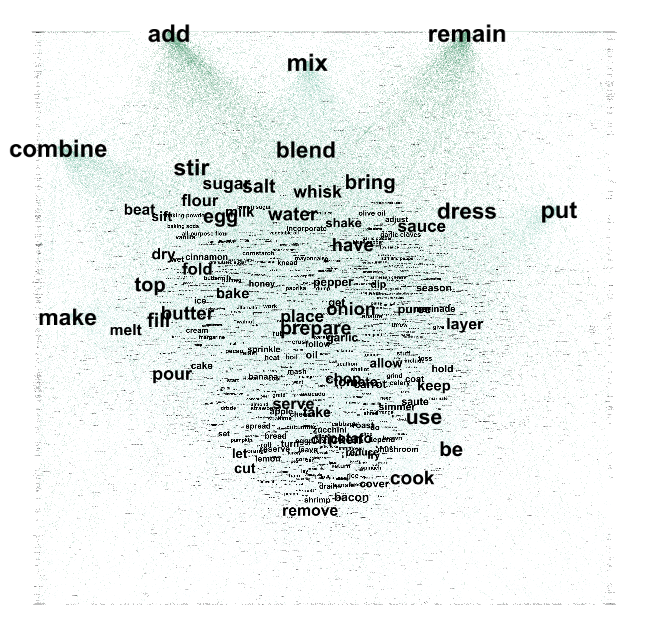
\includegraphics[width=\linewidth]{action-ingredient-graph.png}
	\caption{Grafo Ingrediente-Acción (8223 nodos y 55547 aristas).}
	\label{fig:ingredient-action-graph}
\end{figure}

Dicho de otra forma,

$$w(X, Y) = \frac{|P_{<X,Y>}|}{|P_X \cup P_Y|}$$

Donde $w(X,Y)$ representa el peso de la arista entre la acción $X$ y el ingrediente $Y$, $P_{<X,Y>}$ representa 
el conjunto de los pares $<X,Y>$ y $P_X$ y $P_Y$ representan los pares en los que se encuentra X e Y 
respectivamente.


\subsection{Grafo Receta-Receta}

Se define como un grafo no dirigido en el cual sus nodos representan recetas y sus aristas
están ponderadas con una métrica de similitud entre recetas. Para este tipo de grafo se confeccionaron dos 
versiones basadas en diferentes métricas:

\begin{enumerate}
	\item Similitud de Jaccard entre los conjuntos de ingredientes utilizados por ambas recetas (Figuras \ref{fig:cocina_minuto_recipe_jaccard} y \ref{fig:foodcom_recipe_jaccard}).
	\item Similitud vectorial entre representación semántica de recetas (Figura \ref{fig:foodcom_recipe_semantic}).
\end{enumerate}

\subsubsection{Similitud de Jaccard}

Para la confección de este grafo las aristas son ponderadas mediante la similitud de Jaccard (Ecuación \ref{eq:jaccard_sim}).

\begin{equation}
	J(A, B) = \frac{|A \cap B|}{|A \cup B|}
	\label{eq:jaccard_sim}
\end{equation}

\begin{enumerate}
	\item Se representaron las recetas como el conjunto de ingredientes que se necesitan para ser preparadas.
	\item Se calcula la similitud de Jaccard para cada par de nodos obteniendo el peso de la arista correspondiente.
\end{enumerate}

\subsubsection{Similitud semántica de recetas}

Para la confección de este grafo se realizaron un conjunto de pasos para la vectorización semántica de las recetas.

\begin{enumerate}
	\item Se representaron las recetas como una lista de las instrucciones de su preparación.
	\item Cada instrucción fue codificada por el modelo \textit{Universal Sentence Encoder} \autocite{cer2018universal}
	el cual devuelve un vector de dimensión 512 por cada oración procesada, obteniendo una representación final
	para la receta con dimensión $(CantInstrucciones, 512)$. 
	\item Se procedió a disminuir la dimensión hasta un vector de dimensión 256. Esto se logra mediante un 
	entrenamiento no supervisado con modelo encoder-decoder (Figura \ref{fig:encoder_decoder_small}).
	\item Para el peso de las aristas se utiliza la similitud de exponencial inversa de la distancia entre vectores 
	(Ecuación \ref{eq:inverse_exp_sim})
\end{enumerate}

\begin{equation}
	invExpSim(x, y) = e^{-||x-y||}
	\label{eq:inverse_exp_sim}
\end{equation}

\begin{figure}
	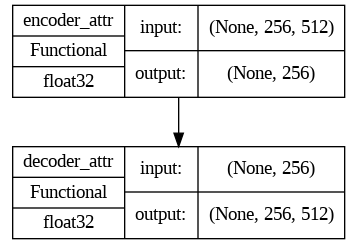
\includegraphics[width=\linewidth]{full_model.png}
	\caption{Arquitectura encoder-decoder para el vectorización de recetas.}
	\label{fig:encoder_decoder_small}
\end{figure}

\subsection{Grafo Ingrediente-Ingrediente}

Se define como un grafo no dirigido en el cual sus nodos representan ingredientes y sus aristas
están ponderadas con una métrica de similitud entre ingredientes. 
Para este tipo de grafo se confeccionaron tres versiones basadas en diferentes métricas:

\begin{enumerate}
	\item Similitud de Jaccard entre los conjuntos de recetas utilizados por ambos ingredientes (Figuras \ref{fig:cocina_minuto_ingredient_jaccard} \ref{fig:foodcom_ingredient_jaccard}).
	\item Similitud vectorial entre representación sintáctica de ingredientes mediante vectorización 
	por frecuencia de términos.
	\item Similitud por \textit{Pointwise mutual information} (PMI) definida en \textcite{teng2012recipe} ((Figuras \ref{fig:cocina_minuto_ingredient_pmi} \ref{fig:foodcom_ingredient_pmi})).
\end{enumerate}

\subsubsection{Similitud de Jaccard}

La confección de este grafo se realiza de manera similar a su contraparte de recetas.

\begin{enumerate}
	\item Los ingredientes se representan por el conjunto de recetas en los que se usan.
	\item Se calcula la similitud de Jaccard (Ecuación \ref{eq:jaccard_sim}) entre ingredientes para ponderar las aristas
	entre estos.
\end{enumerate}

Este grafo provee información acerca de cómo están asociados los ingredientes con las recetas. Una valor de similitud
cercano a 1 indica que los ingredientes pertenecientes a la arista se comparten en la mayoría de las recetas en que son
utilizados. En caso de estar cercano a 0, indica que no coinciden en casi ninguna receta dichos ingredientes.

\subsubsection{Similitud vectorial entre representación sintáctica de ingredientes}

En la confección de este grafo se realiza una transformación del nombre de los ingredientes a vectores mediante
un conteo de las palabras presentes en su nombre.

\begin{enumerate}
	\item Cada ingrediente se representa por su nombre.
	\item Los nombres son vectorizados a una tabla de términos de frecuencia normalizada.
	\item Las aristas entre los ingredientes son ponderadas por la similitud de coseno entre las 
	representaciones vectoriales de cada par de ingredientes.
\end{enumerate}

Una razón por la cual construir este grafo es para dar información acerca de las diferentes variantes de ingredientes.
Estas distintas variantes, por lo general poseen nombres compuestos con la clase principal en su nombre, por ejemplo:

\begin{itemize}
	\item Queso
	\item Queso Parmesano
	\item Queso Ravioli
	\item Queso Gouda
\end{itemize}

\subsubsection{Similitud por PMI}

En la confección de este grafo se calcula el PMI \autocite{teng2012recipe} (Ecuación \ref{eq:pmi}) entre cada par de ingredientes:

\begin{equation}
	PMI(a, b) = \log \frac{p(a,b)}{p(a)p(b)},
	\label{eq:pmi}
\end{equation}

donde

\begin{equation*}
	p(a) = \frac{\text{\# de recetas que contienen \textit{a}}}{\text{\# de recetas}},
\end{equation*}
\begin{equation*}
	p(a,b) = \frac{\text{\# de recetas que contienen \textit{a} y \textit{b}}}{\text{\# de recetas}}.
\end{equation*}

\begin{enumerate}
	\item Cada ingrediente es representado por el conjunto de recetas en el cual es utilizado.
	\item Se calcula el PMI entre cada par de ingredientes y se pondera la arista con este valor.
\end{enumerate}

En este grafo, los pesos pueden llegar a ser negativos o positivos. En este caso nos interesa los pesos positivos,
ya que estos pesos indican que la probabilidad de que coincidan dos ingredientes al mismo tiempo es mayor que la
probabilidad que coincidan de forma independiente, por lo tanto su ocurrencia está condicionada a ser más probable
dado que tengo un ingrediente.

$$
PMI(a,b) = \log \frac{p(a,b)}{p(a)p(b)} > 0
$$
$$
\frac{p(a,b)}{p(a)p(b)} > 1
$$
$$
p(a,b) > p(a)p(b)
$$
$$
p(a|b)p(b) > p(a)p(b) \quad p(b|a)p(a) > p(a)p(b)
$$
$$
p(a|b) > p(a) \quad p(b|a) > p(b)
$$

\section{Ranking}

El ranking se lleva a cabo para tomar la información más relevante de los datos de acuerdo a un criterio.
Se emplea para dos funcionalidades, disminuir la cantidad de los nodos de los grafos y recuperar los elementos
más similares a una consulta dada de los datos.
	
\subsection{Ranking de Nodos}

Dada la cantidad de nodos presentes en los grafos, en algunas situaciones existe la necesidad de reducir esta
cantidad. Para esto se toman diferentes estrategias en dependencia del tipo de grafo con el que se trabaje:

\begin{enumerate}
	\item Ranking de recetas por valoraciones de usuarios.
	\item Ranking de ingredientes por ocurrencias acumuladas.
\end{enumerate}

\subsubsection{Ranking de recetas por valoraciones de usuarios}

Dado un conjunto de valoraciones a recetas dadas por usuarios se procede a definir 
una medida de importancia con estas. Para esto se realizan los siguintes pasos:

\begin{enumerate}
	\item Se extraen para cada receta la cantidad de valoraciones y la media de estas.
	\item Dichos valores son normalizados entre 0 y 1 al dividirlos por la cantidad máxima de ambas métricas por receta.
	\item Se calcula la métrica F1 entre ambos valores para obtener la importancia final de la receta (Ecuación \ref{eq:f1_recipe_rank}).
\end{enumerate}

\begin{equation}
	ImpReceta(r, Val) = F1(A(r, Val), M(r, Val)),
	\label{eq:f1_recipe_rank}
\end{equation}

donde

\begin{equation*}
	F1(a, b) = 2 \frac{a · b}{a + b},
\end{equation*}

\begin{equation*}
	A(r, Val) = \frac{|[r \sqsubseteq Val]|}{\max \{\,|[p \sqsubseteq Val]| \, \vert \, p \in R \, \}},
\end{equation*}

\begin{equation*}
	M(r, Val) = \frac{mean([r \sqsubseteq Val])}{\max \{\,mean([p \sqsubseteq Val]) \, \vert \, p \in R\,\}},
\end{equation*}

$Val$ es la lista de valoraciones dadas por los usuarios, la expresión $[r \sqsubseteq Val]$ denota la lista de valores de 
las valoraciones dadas a la receta $r$ y $R$ es el conjunto de recetas.

Esta métrica previene que recetas con pocas y muy altas valoraciones tengan más importancia que recetas con muchas
valoraciones pero más bajas. De manera que las recetas más importantes tengan que tener al mismo tiempo una gran 
cantidad de valoraciones y que estas sean buenas (Figura \ref{fig:f1_plot}).

Este algoritmo fue utilizado para reducir el número de recetas de Food.com para la construcción de los grafos 
tipo Receta-Receta. La reducción se hizo a 5000 nodos dado que a partir de esta cantidad la relevancia de las
recetas es muy baja (Figura \ref{fig:recipe_user_ranking_info})

\subsubsection{Ranking de ingredientes por ocurrencias acumuladas}

Dado un conjunto de ingredientes se toman los que participan en la mayor cantidad de enlaces entre recetas.
Para realizar el ranking se realizan los siguientes pasos:

\begin{enumerate}
	\item Ordenar por grado de mayor a menor los nodos ingredientes del grafo bipartito de ingredientes-recetas.
	\item Seleccionar los ingredientes, por este orden, hasta que la suma de los grados de los nodos seleccionados 
	represente un porciento fijo de la suma total de todos los grados del grafo.
\end{enumerate}

Este algoritmo fue utilizado para reducir el número de ingredientes de Food.com para la construcción de los grafos 
tipo Ingrediente-Ingrediente. Los ingredientes resultantes contiene un 90\% de las ocurrencias
con solo 521 lo que representa solo el 3.5\% del total (Figura \ref{fig:ingredient_degree_ranking_info})

\subsection{Ranking de Resultados a Consultas}
\label{subsec:rank_query}

Para la extracción de ingredientes y recetas dadas una consulta se emplean dos mecanismos para hacer el cálculo
de la relevancia.

\begin{itemize}
	\item Distancia de Levenshtein: Se calcula la distancia de Levenshtein entre la consulta y el nombre de la 
	entidad a extraer.
	\item Similitud Vectorial: Se calcula la similitud de coseno entre la vectorización de la consulta y los
	vectores de la entidad. Las entidades son vectorizadas mediante una tabla TF-IDF. 
	\item Ranking de recetas por ingredientes que las usen.
\end{itemize}

\subsubsection{Ranking de recetas por ingredientes que las usen}

Dado un conjunto de ingredientes se quiere encontrar las recetas que los usen, para esto se toman dos variantes.
En primer lugar se ordena por la cantidad de ingredientes que tienen las recetas en común con los ingredientes
requeridos. Esta aproximación lleva a que en casos de que la intersección sea completa se ordene por nombre lo que
no necesariamente es deseable. El otro método es vectorizar las recetas por sus ingredientes mediante TF-IDF y
realizar el ranking con la similitud de coseno entre la vectorización TF-IDF de los ingredientes consultados.

\section{Motor de Búsqueda}

Para la confección del motor de búsqueda de recetas se conformó un paquete de Python, \textbf{recipy}, el cual
contiene las funciones necesarias para la creación y consulta de grafos. Para la visualización de los
resultados se creó una aplicación usando \textbf{streamlit} la cual permite al usuario interactuar con la API.

En este el usuario puede hacer distintas consultas a los distintos grafos para recuperar la información deseada.

\subsection{Métodos de Búsqueda}

Para los algoritmos funcionen es conveniente tener el nodo exacto sobre el cual se realiza la consulta. Para la
obtención de dicho nodo a partir de una consulta de texto se emplean los métodos explicados en la sección 
\nameref{subsec:rank_query} para la obtención de un ranking de posibles candidatos. Con este resultado el usuario
puede seleccionar el más adecuado y con esta información realizar la consulta a un nodo concreto.

\subsection{Consultas}

La aplicación provee al usuario de un conjunto de consultas predefinidas.

\subsubsection{Buscar recetas por nombre}

Dado una consulta devuelve las primeras mejores 100 recetas de acuerdo al criterio de búsqueda seleccionado
(Figura \ref{fig:recipe_search_tfidf}).
Esta consulta se realiza sobre el grafo bipartito de receta-ingrediente, filtrando los nodos recetas. 

\subsubsection{Buscar ingredientes por nombre y ver recetas que los usan}

Dado una consulta devuelve los primeros mejores 100 ingredientes de acuerdo al criterio de búsqueda seleccionado,
estos ingredientes luego pueden ser añadidos a una canasta de la cual se seleccionaran los ingredientes para hacer
la búsqueda de recetas con estos, devolviendo los mejores 100 resultados de acuerdo al segundo criterio seleccionado
(Figura \ref{fig:ingredient_search_tfidf}).
Ambas partes de la consulta se realizan sobre el grafo bipartito de receta-ingrediente, filtrando los nodos 
ingredientes en la primera y calculando las métricas correspondientes en la segunda.

\subsubsection{Buscar ingrediente que mezcle bien con otro}

Dado una consulta devuelve los primeros mejores 100 ingredientes de acuerdo al criterio de búsqueda seleccionado,
estos ingredientes luego pueden ser seleccionados, devolviendo los mejores 100 ingredientes con los cuales se puede 
complementar (Figura \ref{fig:complementary_ingredient_search_tfidf}). Esta consulta es realizada sobre el grafo 
PMI de ingredientes.

\subsubsection{Buscar recetas por similitud entre estas}

La similitud entre recetas se viene dada de dos formas:

\begin{itemize}
	\item Por coincidencia de ingredientes: En este caso se devuelven las que tengan mayores conincidencias
	con la receta dada. Calculando dichas recetas por el grafo bipartito de ingrediente-recetas (Figura \ref{fig:recipe_ingredient_tfidf}). 
	\item Por similitud semántica: En este caso se devuelven las recetas ordenadas por pesos adyacentes
	a la receta dada en el grafo de similitud semántica (Figura \ref{fig:recipe_semantic_tfidf}).
\end{itemize}

\subsubsection{Reemplazo de ingredientes}

Dado un ingrediente, es posible hacer una lista ordenada de aquellos otros por los que puede ser sustituido. 
Esto se logra tomando la partición del grafo \emph{ingrediente-ingrediente} a la cual pertenece el ingrediente 
dado para obtener una lista de posibles reemplazos. Luego, se ordenan estos de acuerdo al índice de Jaccard de 
la cantidad de acciones comunes entre ambos ingredientes, utilizando el grafo de $<$acción, ingrediente$>$. De 
esta forma se obtiene una medida, para cada elemento de la lista obtenida, de cuan seguro es usar dicho 
ingrediente como reemplazo del original. 

Se implementó una herramienta usando streamlit mediante la cual el usuario inserta un ingrediente en un cuadro 
de texto y se le muestra una lista con los elementos por los cuales puede ser sustituido 
(Figura \ref{fig:ingredient-replacement}).

\section{Conclusiones}

En este trabajo se estudió e implementó una herramienta informática para la extracción de información relevante 
del dataset de recetas Food.com a partir del uso de diversos algoritmos de Inteligancia Artificial, Sistemas de 
Recuperación de Información y Análisis de Redes Complejas. En particular, se construyeron diversos sistemas 
complejos a partir de las relaciones existentes entre los ingredientes, las recetas, los pasos de preparación y 
los \textit{reviews} de usuarios existentes en el dataset mencionado, a partir de los cuales fue posible realizar 
consultas como: Qué ingredientes puede sustituir un ingrediente dado?, Qué recetas puedo elaborar dada esta lista 
de ingredientes?, Qué recetas son similares a una receta dada?, entre otros.

%----------------------------------------------------------------------------------------
%	 REFERENCES
%----------------------------------------------------------------------------------------

\printbibliography % Output the bibliography

%----------------------------------------------------------------------------------------


%----------------------------------------------------------------------------------------
%	 ANEXOS
%----------------------------------------------------------------------------------------
\section{Anexos}

\newpage

\begin{figure}
	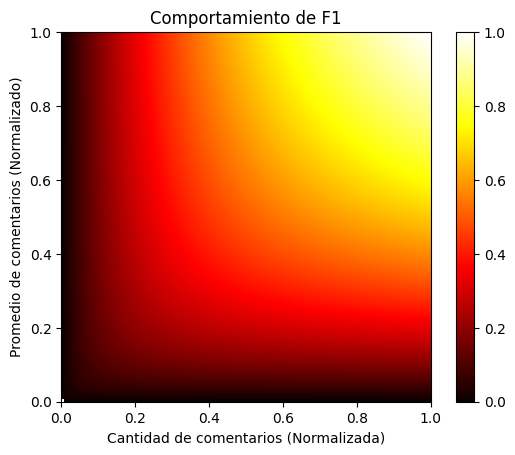
\includegraphics[width=\linewidth]{f1_image.png}
	\caption{Variación del valor de F1 en dependencia de los argumentos.}
	\label{fig:f1_plot}
\end{figure}

\begin{figure}
	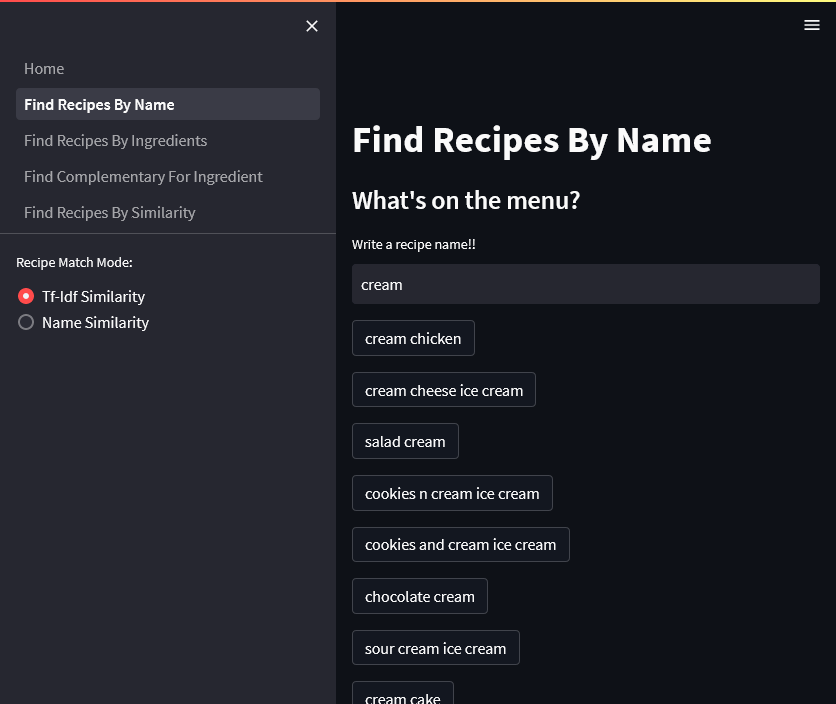
\includegraphics[width=\linewidth]{find_recipe_streamlit.png}
	\caption{Búsqueda de receta por nombre con ranking TF-IDF.}
	\label{fig:recipe_search_tfidf}
\end{figure}

\begin{figure}
	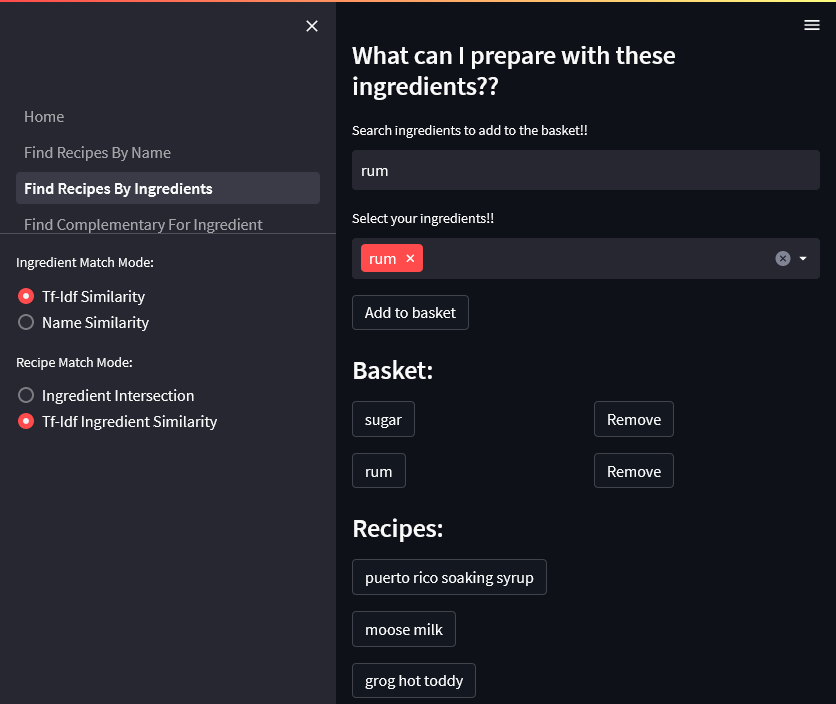
\includegraphics[width=\linewidth]{find_ingredient_streamlit.png}
	\caption{Búsqueda de ingredientes por nombre con ranking TF-IDF y de recetas para realizar con estos.}
	\label{fig:ingredient_search_tfidf}
\end{figure}

\begin{figure}
	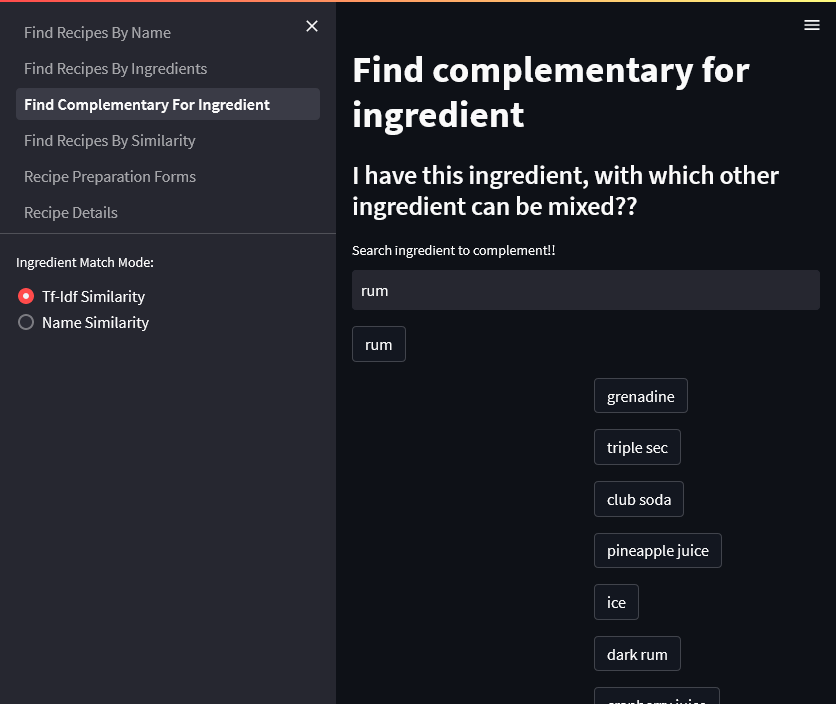
\includegraphics[width=\linewidth]{find_complementary_ingredient_streamlit.png}
	\caption{Búsqueda de ingredientes para complementar un ingrediente dado.}
	\label{fig:complementary_ingredient_search_tfidf}
\end{figure}

\begin{figure}
	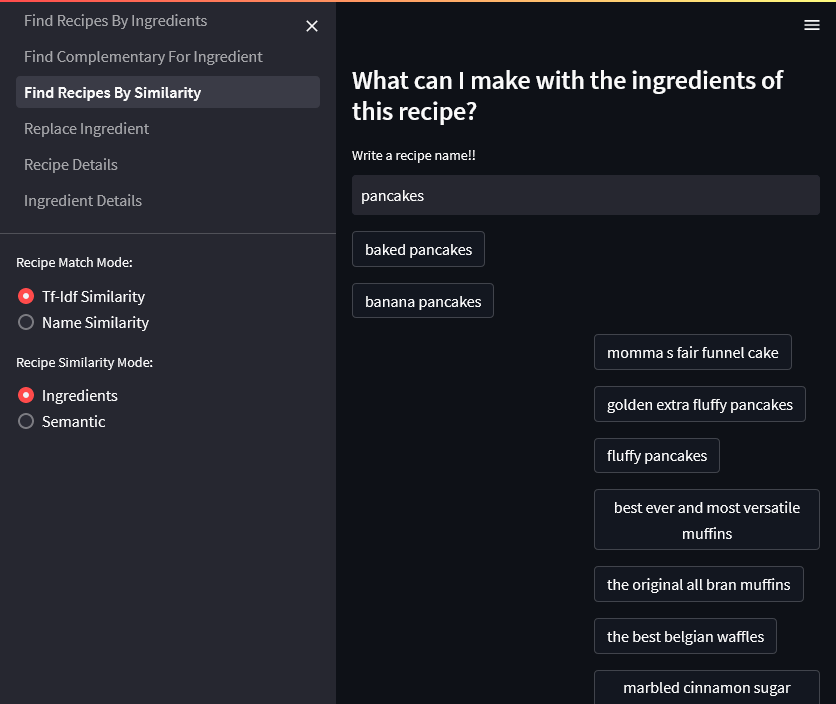
\includegraphics[width=\linewidth]{find_recipe_ingredient_streamlit.png}
	\caption{Búsqueda de ingredientes para complementar un ingrediente dado.}
	\label{fig:recipe_ingredient_tfidf}
\end{figure}

\begin{figure}
	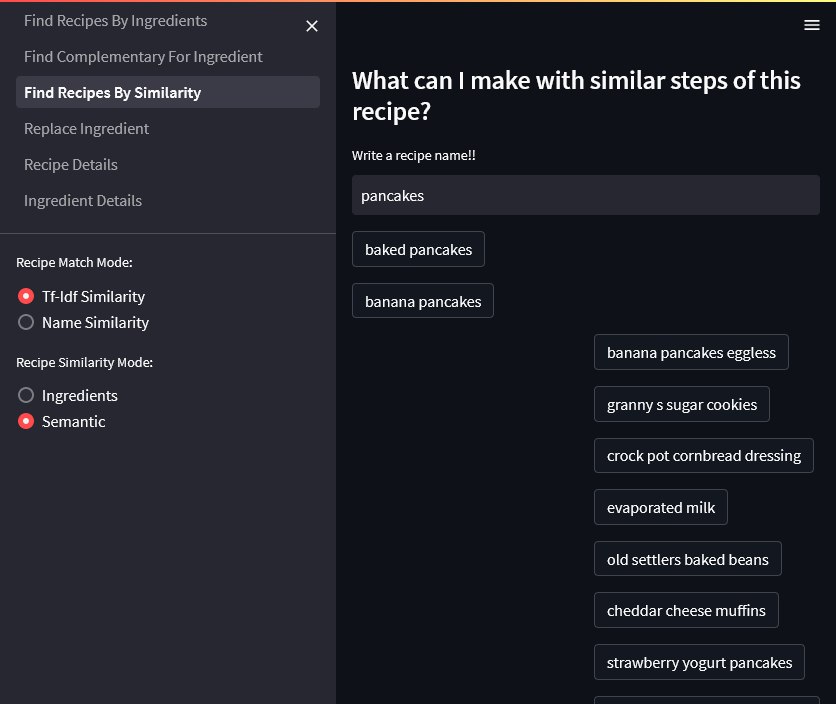
\includegraphics[width=\linewidth]{find_recipe_semantic_streamlit.png}
	\caption{Búsqueda de ingredientes para complementar un ingrediente dado.}
	\label{fig:recipe_semantic_tfidf}
\end{figure}

\begin{figure}
	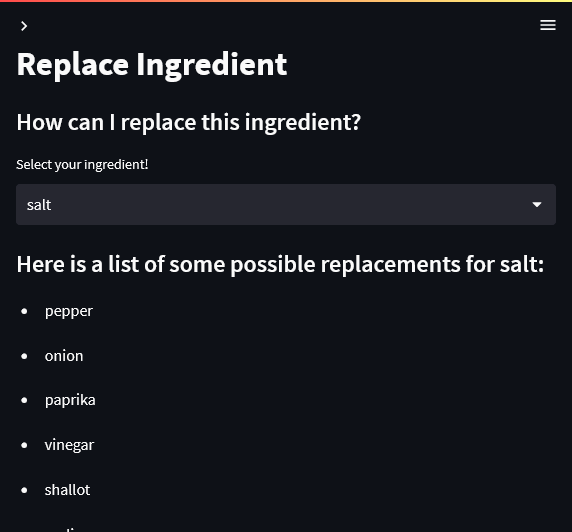
\includegraphics[width=\linewidth]{ingredient-replacement.png}
	\caption{Página de reemplazo de ingredientes.}
	\label{fig:ingredient-replacement}
\end{figure}

\begin{figure} % Single column figure
	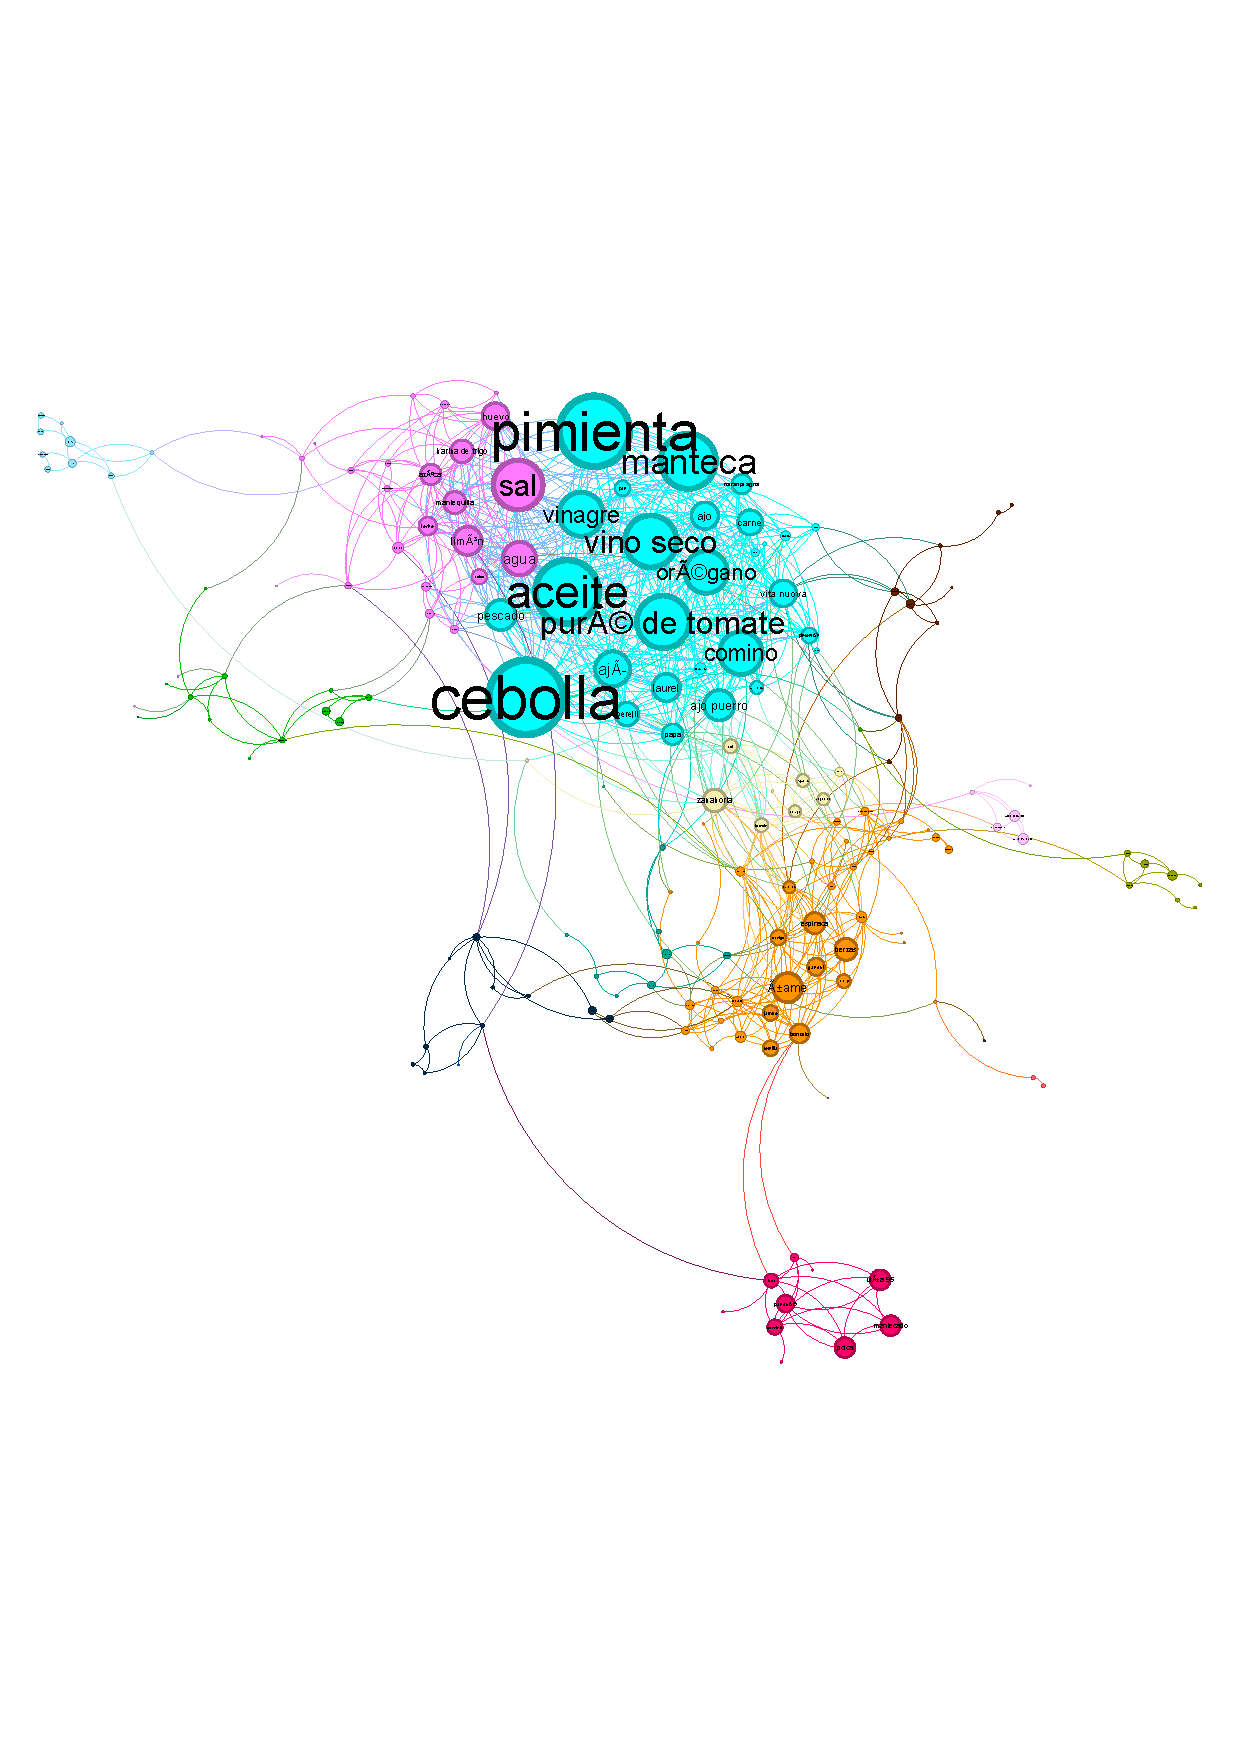
\includegraphics[width=\linewidth]{cocina_minuto/ingredient_node_jaccard_weighted.pdf}
	\caption{Cocina al Minuto Grafo Ingrediente-Ingrediente ponderado con Similitud de Jaccard entre Recetas.}
	\label{fig:cocina_minuto_ingredient_jaccard}
\end{figure}

\begin{figure} % Single column figure
	\includegraphics[width=\linewidth]{cocina_minuto/ingredient_node_pmi_weighted.pdf}
	\caption{Cocina al Minuto Grafo Ingrediente-Ingrediente ponderado con Métrica de PMI entre Recetas.}
	\label{fig:cocina_minuto_ingredient_pmi}
\end{figure}

\begin{figure} % Single column figure
	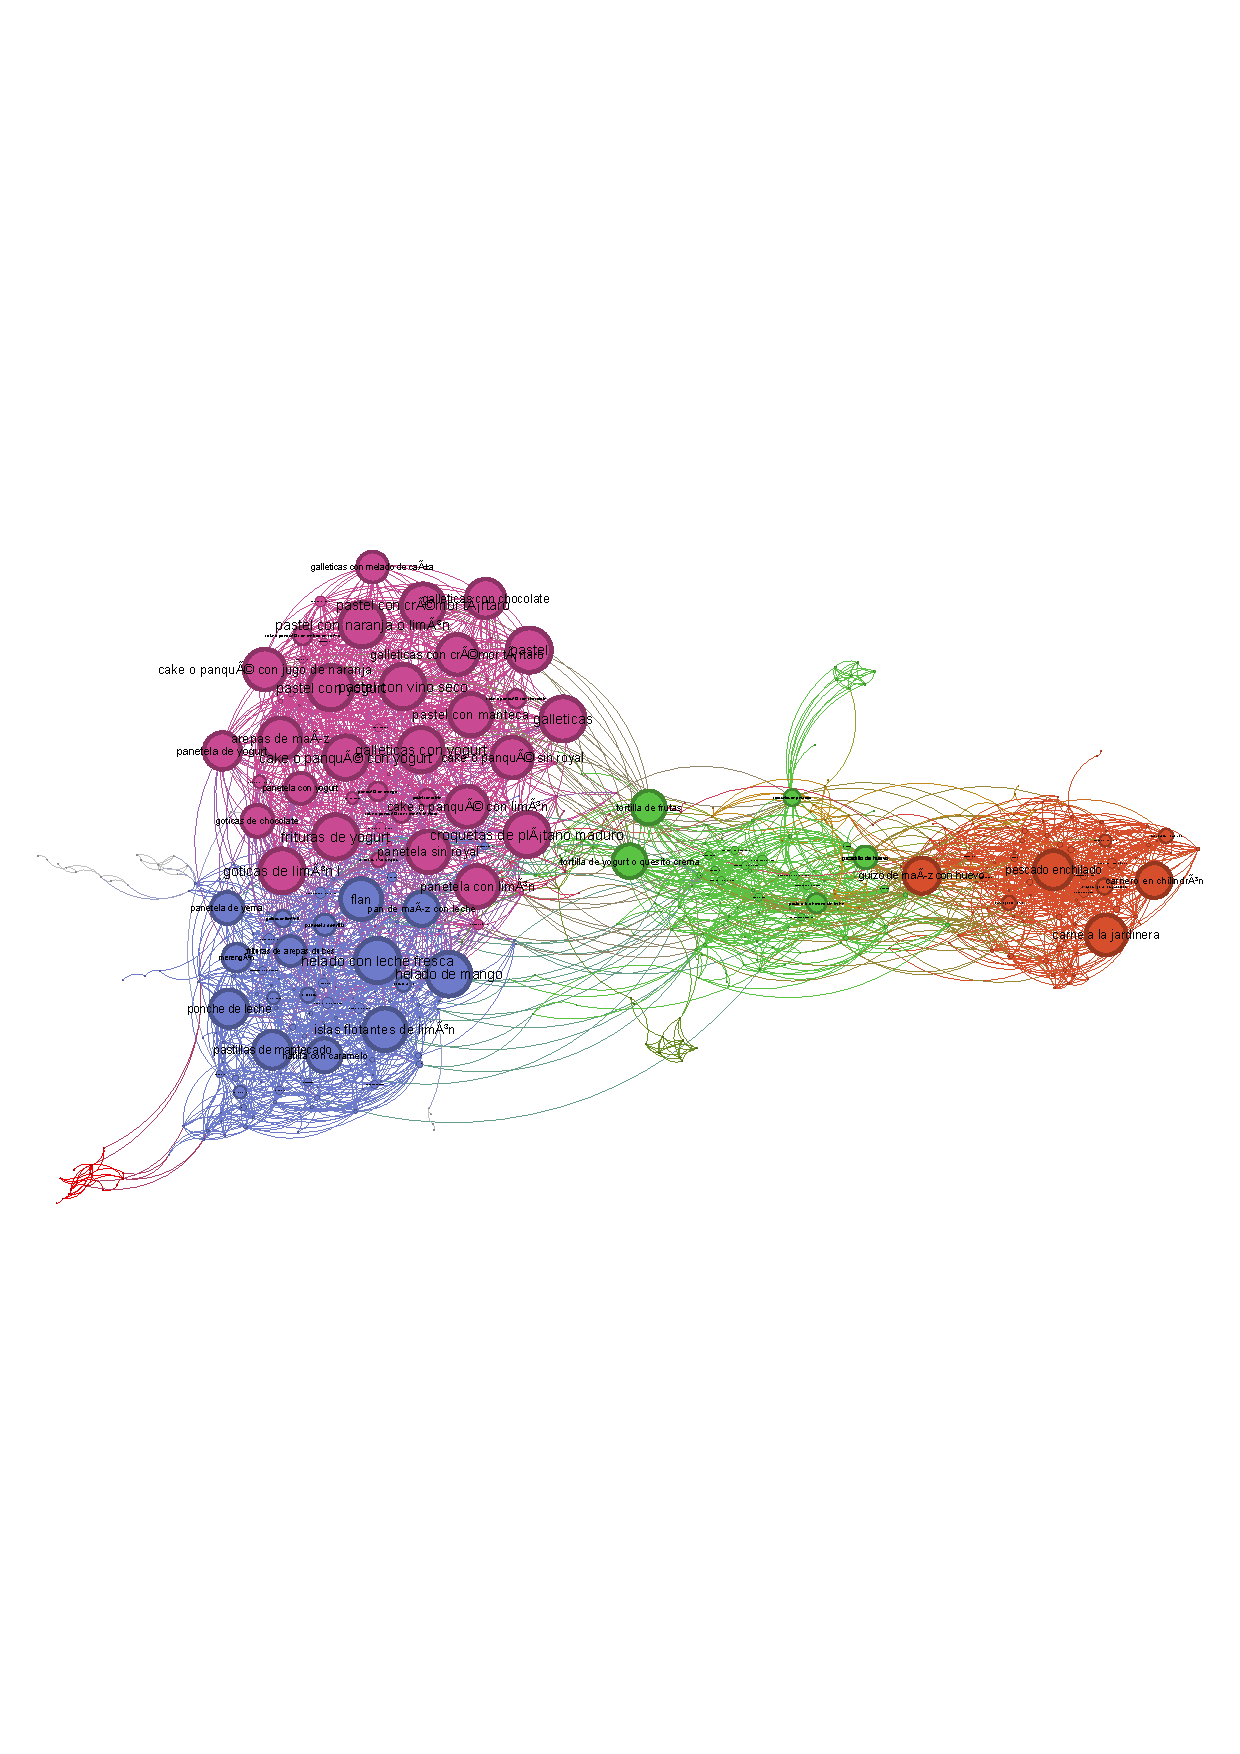
\includegraphics[width=\linewidth]{cocina_minuto/recipe_node_weighted.pdf}
	\caption{Cocina al Minuto Grafo Receta-Receta ponderado con Similitud de Jaccard entre Ingredientes.}
	\label{fig:cocina_minuto_recipe_jaccard}
\end{figure}


\begin{figure} % Single column figure
	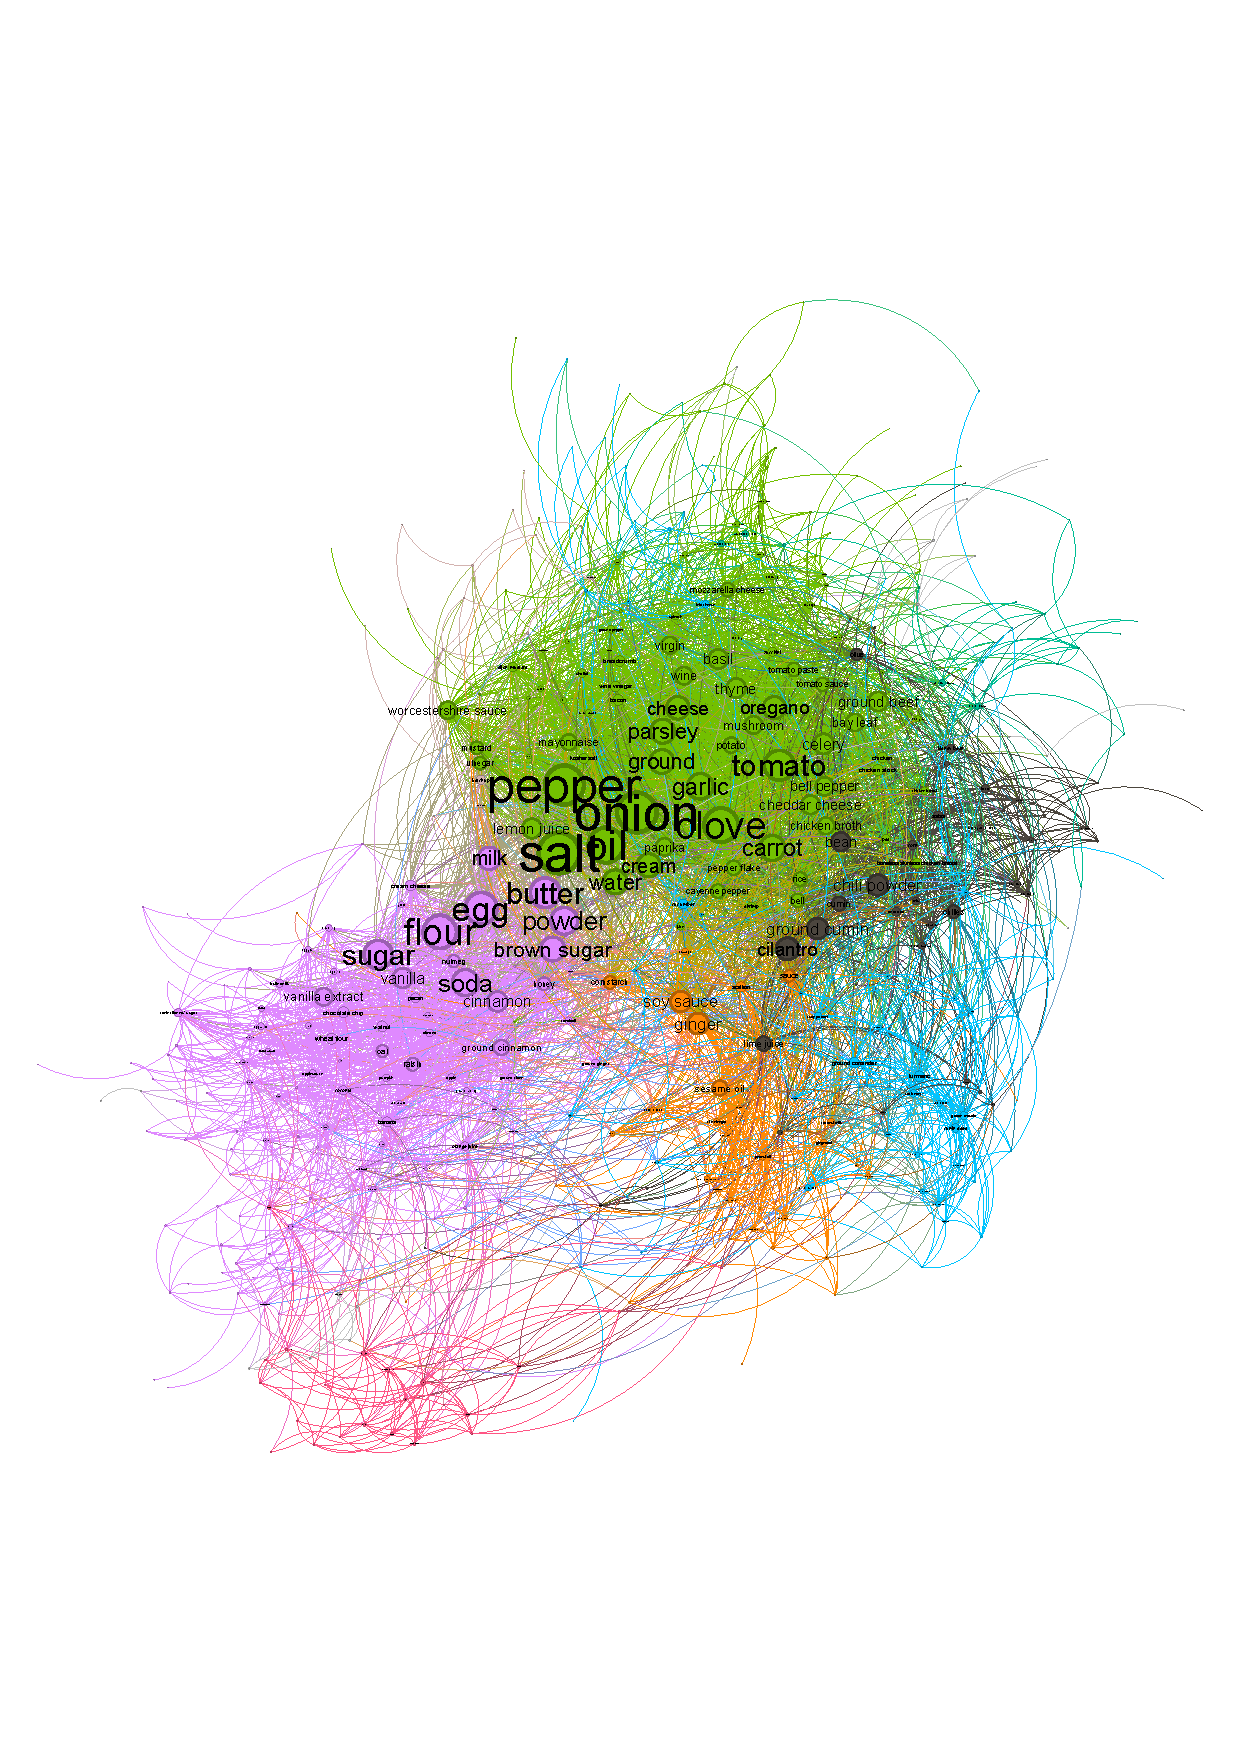
\includegraphics[width=\linewidth]{foodcom/ingredient_node_weighted_foodcom.pdf}
	\caption{Food.com Grafo Ingrediente-Ingrediente ponderado con Similitud de Jaccard entre Recetas.}
	\label{fig:foodcom_ingredient_jaccard}
\end{figure}

\begin{figure} % Single column figure
	\includegraphics[width=\linewidth]{foodcom/ingredient_node_pmi_weighted.pdf}
	\caption{Food.com Grafo Ingrediente-Ingrediente ponderado con Métrica de PMI entre Recetas.}
	\label{fig:foodcom_ingredient_pmi}
\end{figure}

\begin{figure} % Single column figure
	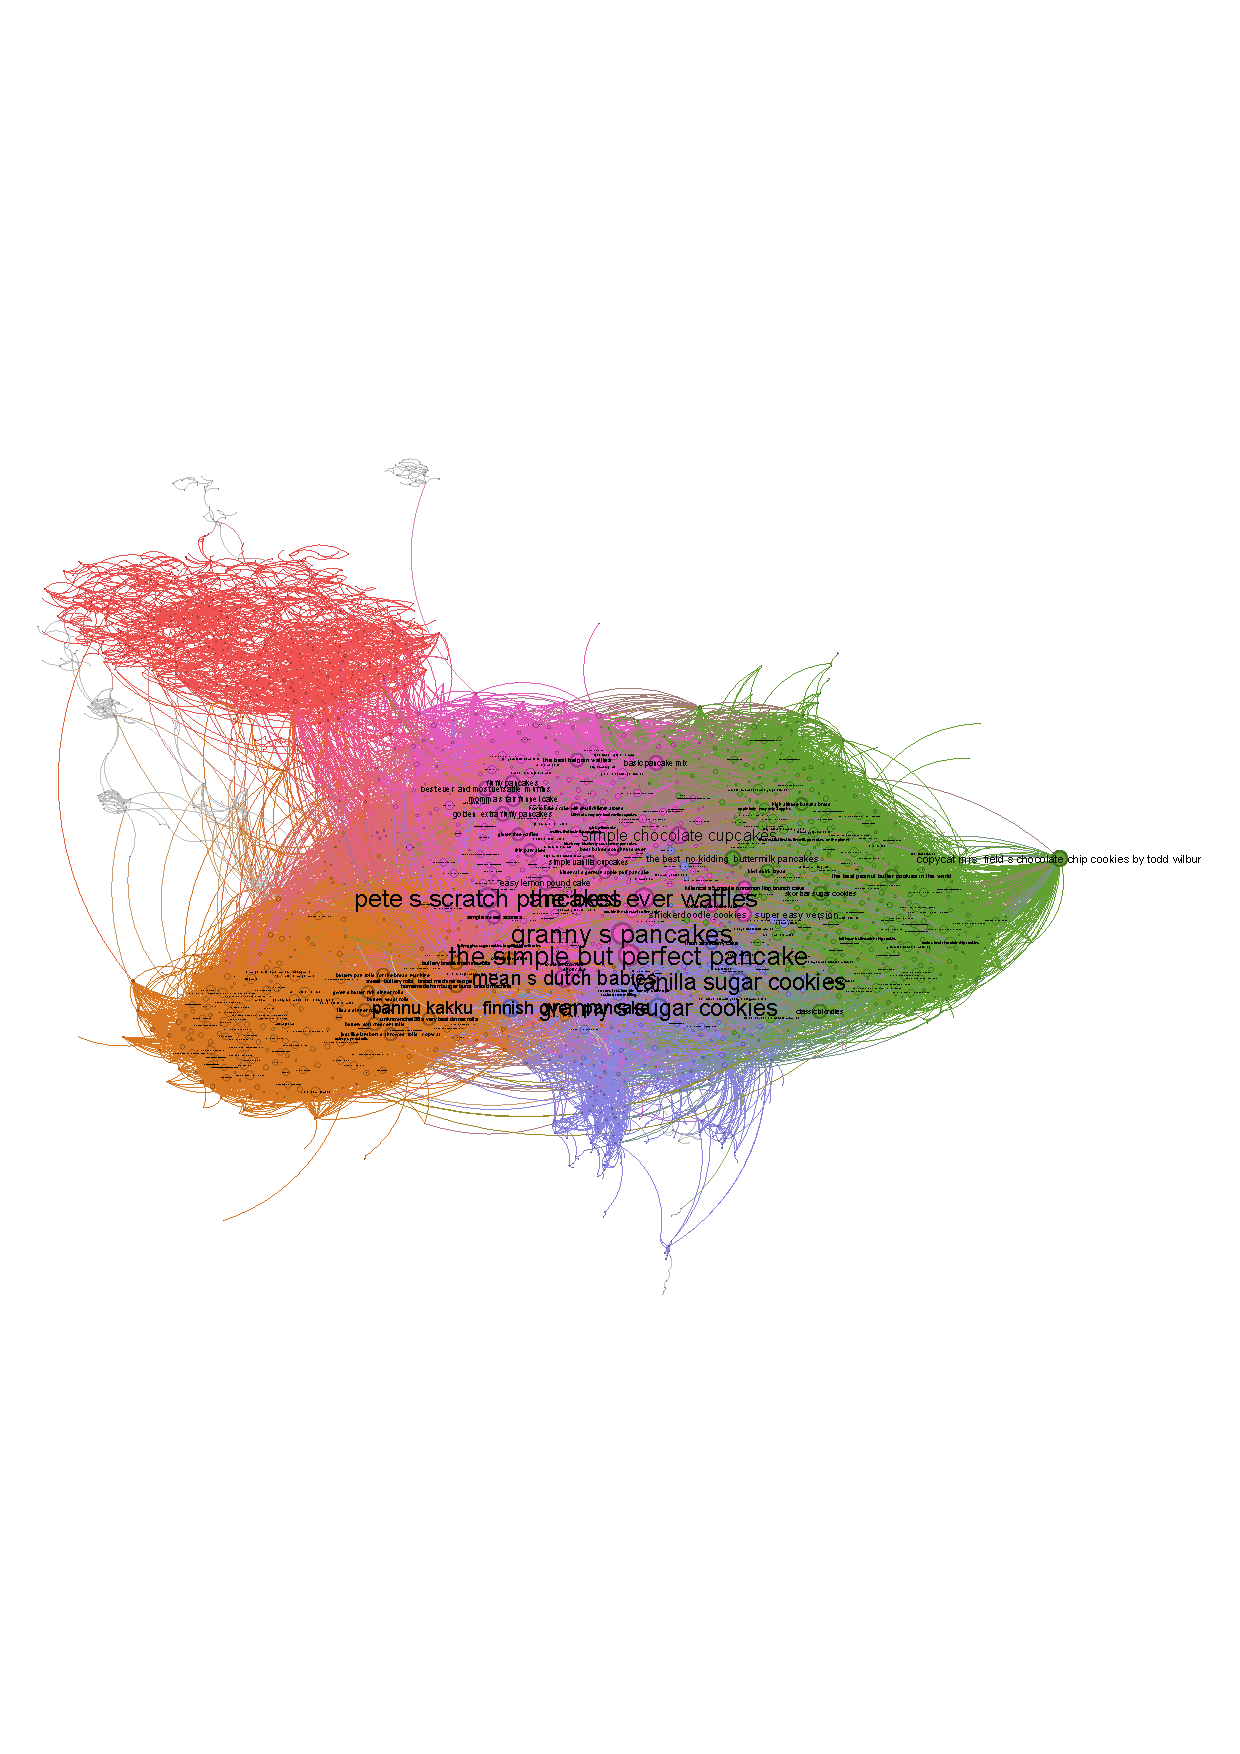
\includegraphics[width=\linewidth]{foodcom/recipe_node_weighted_reduced_5000.pdf}
	\caption{Food.com Grafo Receta-Receta ponderado con Similitud de Jaccard entre Ingredientes.}
	\label{fig:foodcom_recipe_jaccard}
\end{figure}

\begin{figure} % Single column figure
	\includegraphics[width=\linewidth]{foodcom/recipe_node_semantic_weighted.pdf}
	\caption{Food.com Grafo Receta-Receta ponderado con Similitud Semántica entre Recetas.}
	\label{fig:foodcom_recipe_semantic}
\end{figure}

\begin{figure*}
	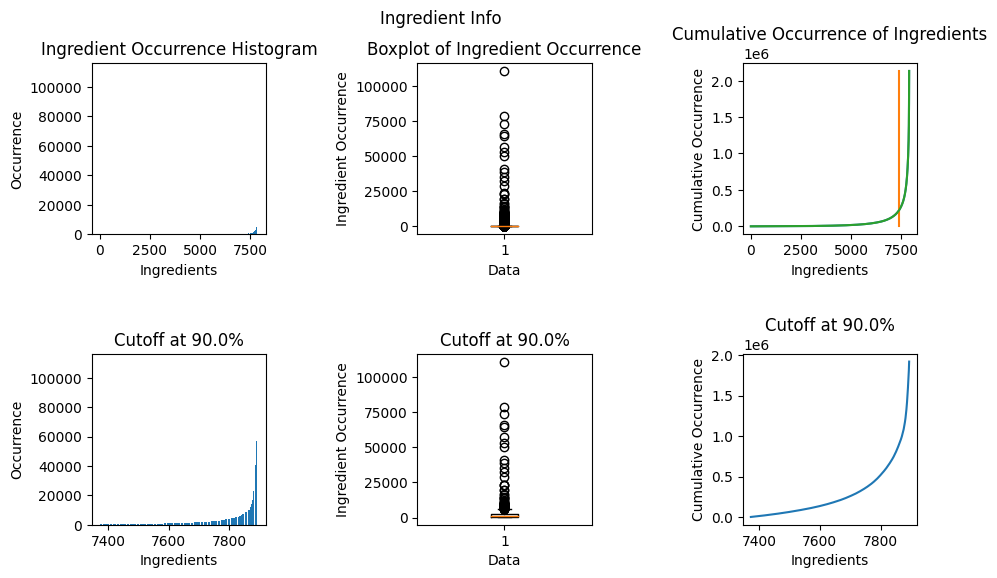
\includegraphics[width=\linewidth]{ingredient_degree_ranking_info.png}
	\caption{Reporte de importancia de los ingredientes dado la cantidad de veces que son usados en las recetas.}
	\label{fig:ingredient_degree_ranking_info}
\end{figure*}

\begin{figure*}
	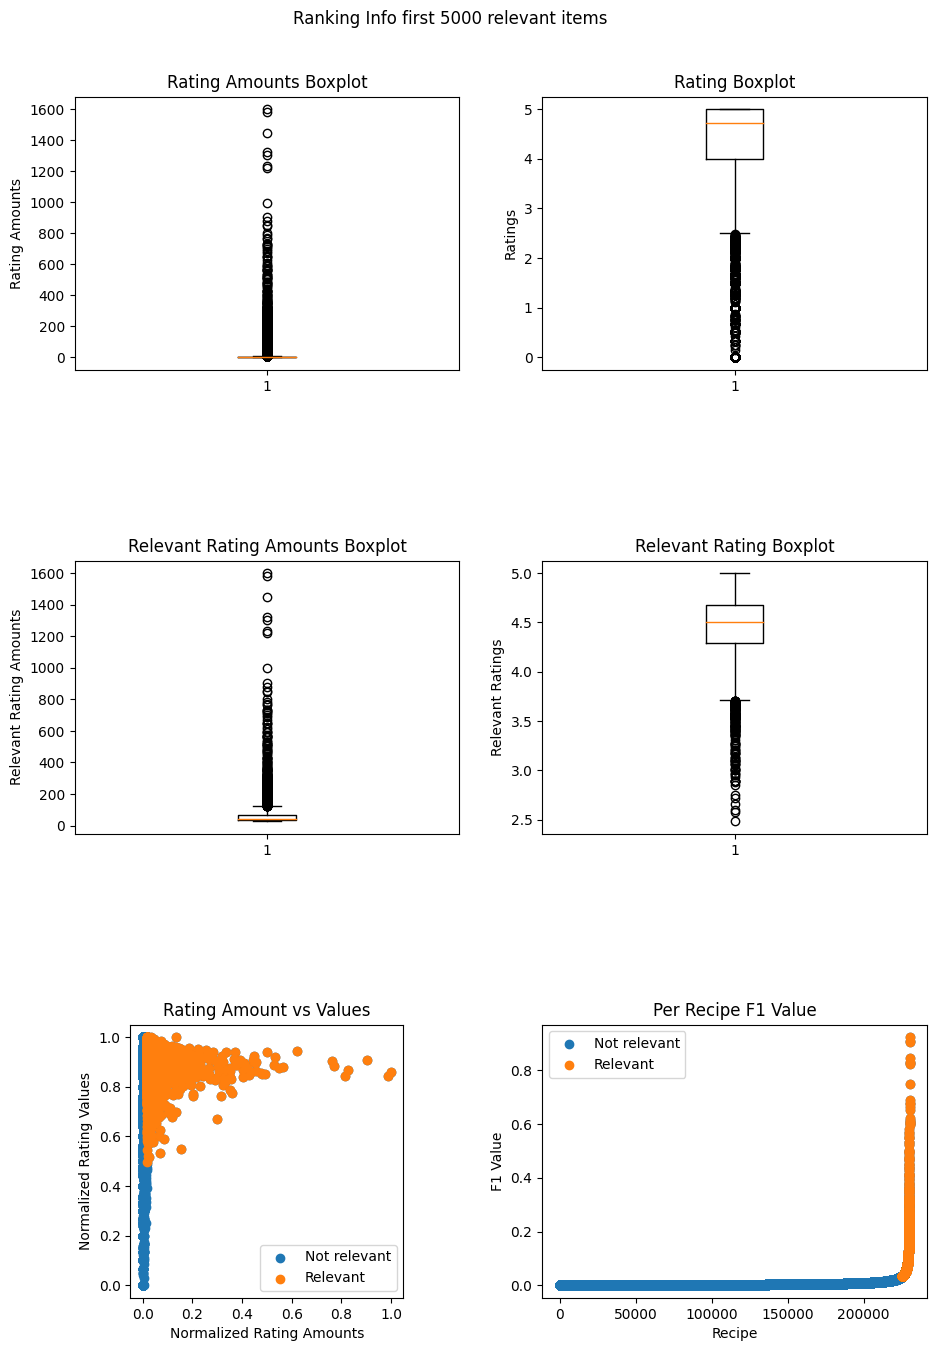
\includegraphics[width=\linewidth]{recipe_user_ranking_info.png}
	\caption{Reporte de importancia de las recetas dada la métrica F1.}
	\label{fig:recipe_user_ranking_info}
\end{figure*}

\begin{figure*}
	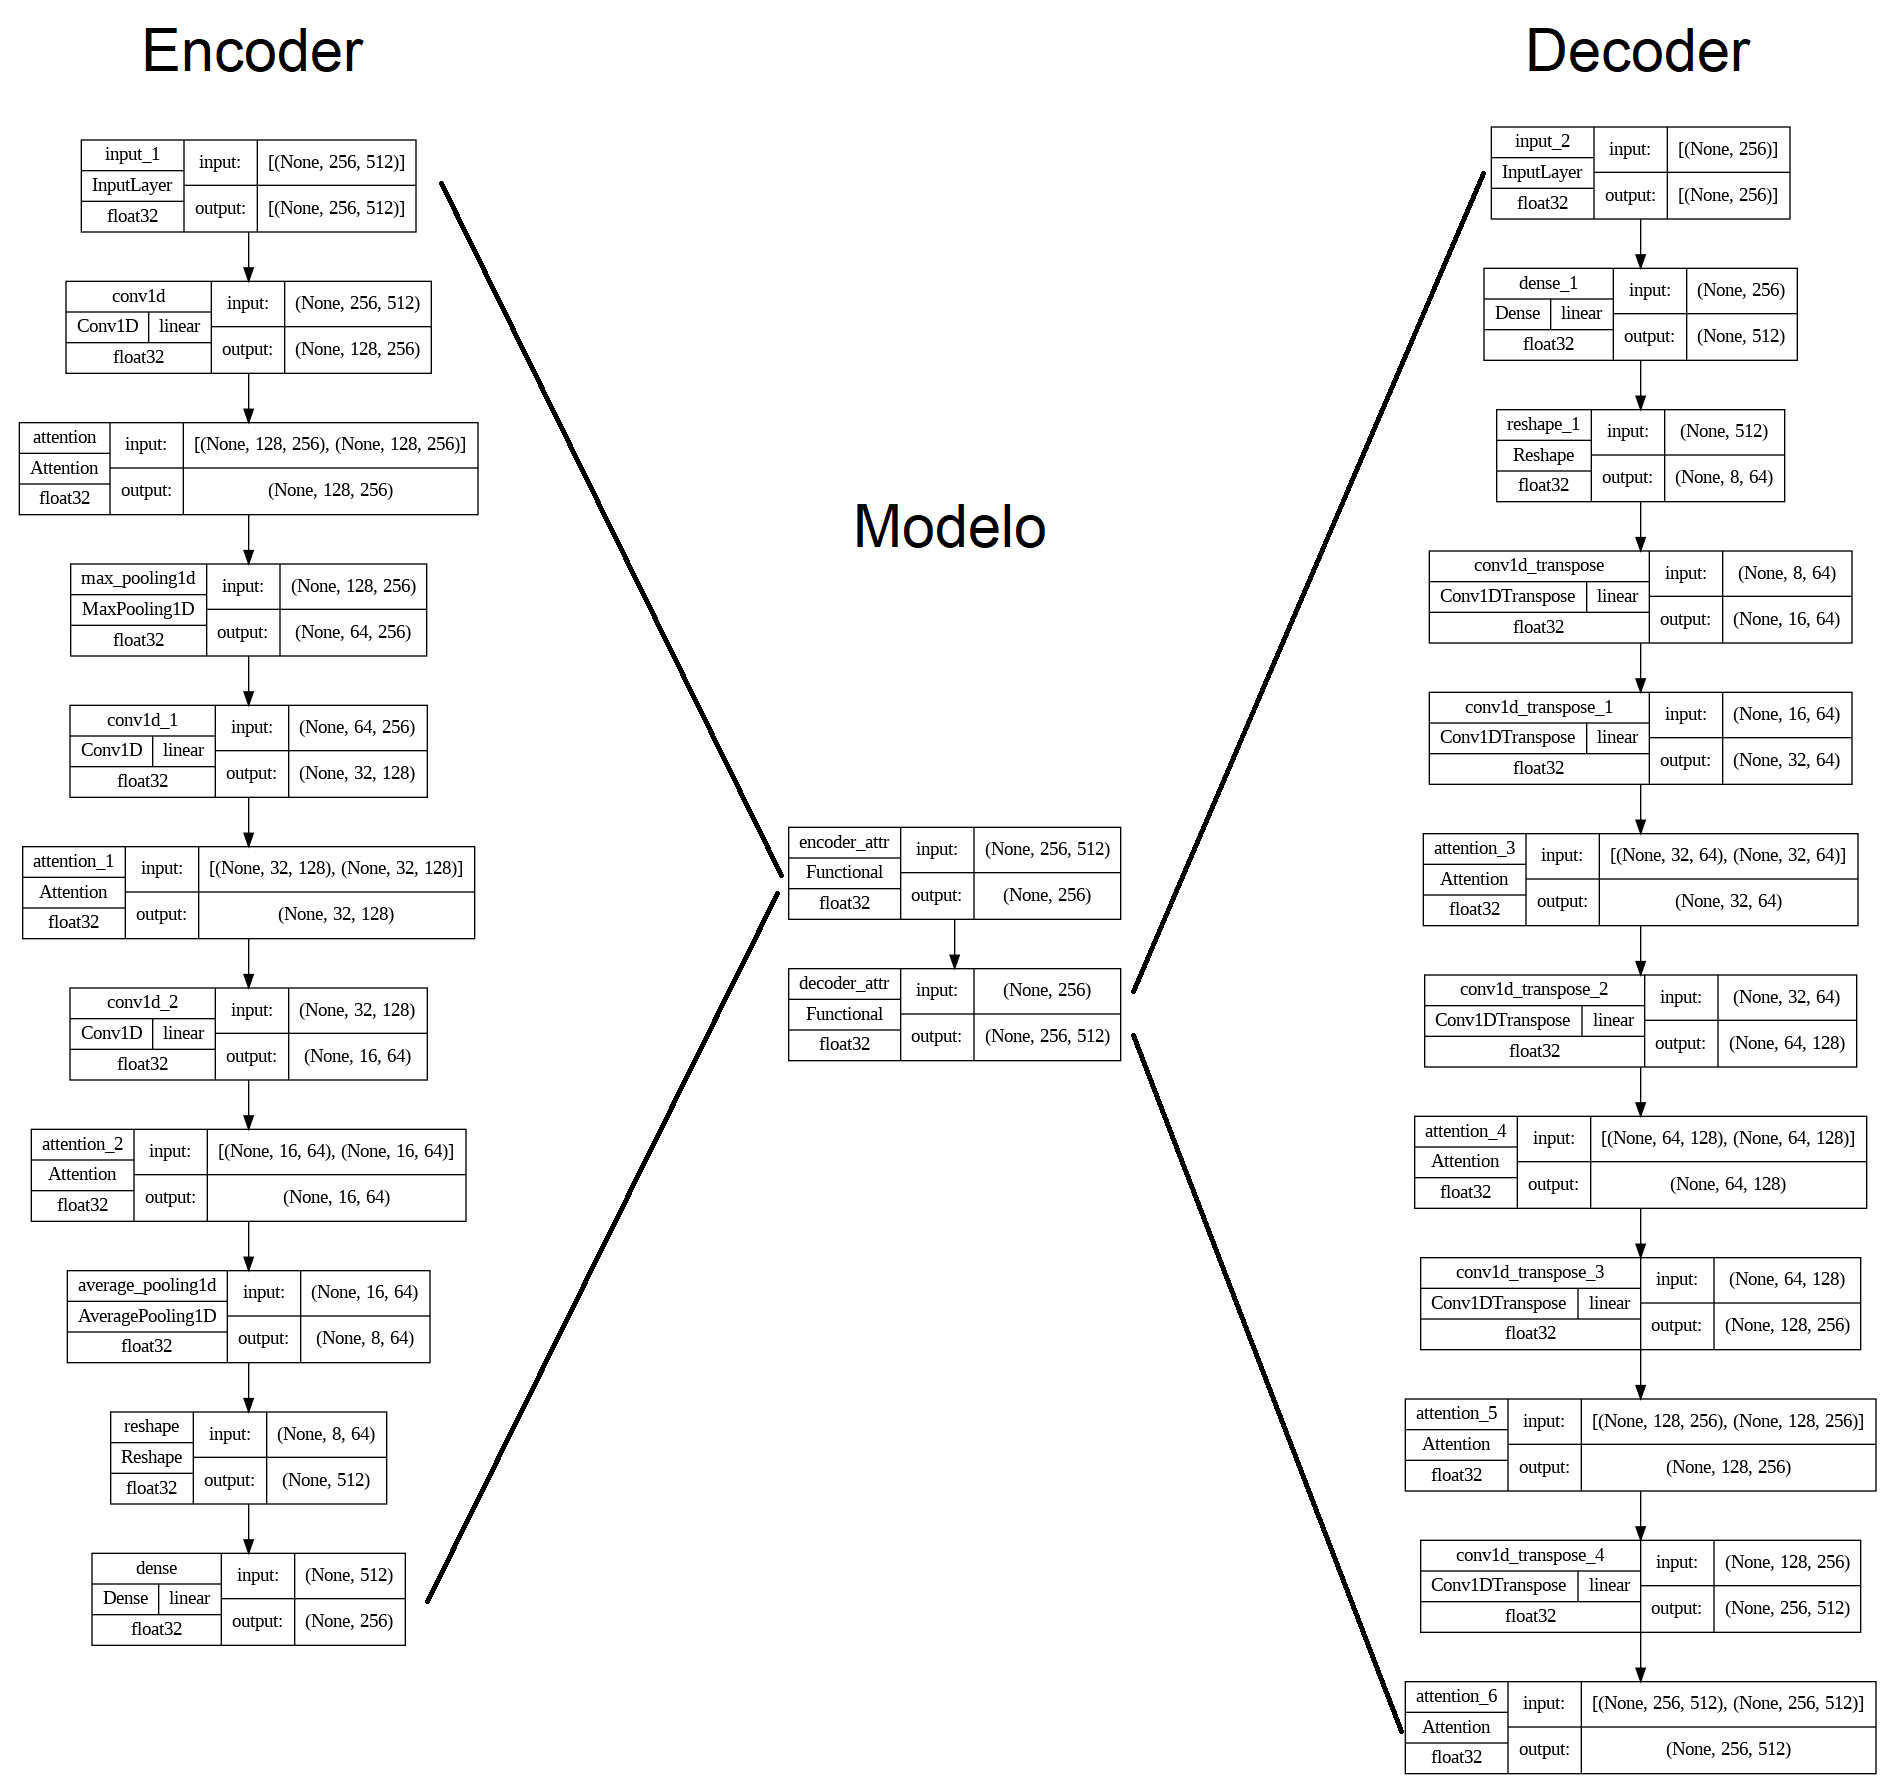
\includegraphics[width=\linewidth]{architecture.png}
	\caption{Arquitectura encoder-decoder para el vectorización de recetas.}
	\label{fig:encoder_decoder}
\end{figure*}

%----------------------------------------------------------------------------------------

\end{document}


% \section{Results}

% \begin{table} % Single column table
% 	\caption{Example single column table.}
% 	\centering
% 	\begin{tabular}{l l r}
% 		\toprule
% 		\multicolumn{2}{c}{Location} \\
% 		\cmidrule(r){1-2}
% 		East Distance & West Distance & Count \\
% 		\midrule
% 		100km & 200km & 422 \\
% 		350km & 1000km & 1833 \\
% 		600km & 1200km & 890 \\
% 		\bottomrule
% 	\end{tabular}
% 	\label{tab:distcounts}
% \end{table}

% Referencing a table using its label: Table \ref{tab:distcounts}.

% \begin{table*} % Full width table (notice the starred environment)
% 	\caption{Example two column table with fixed-width columns.}
% 	\centering % Horizontally center the table
% 	\begin{tabular}{L{0.2\linewidth} L{0.2\linewidth} R{0.15\linewidth}} % Manually specify column alignments with L{}, R{} or C{} and widths as a fixed amount, usually as a proportion of \linewidth
% 		\toprule
% 		\multicolumn{2}{c}{Location} \\
% 		\cmidrule(r){1-2}
% 		East Distance & West Distance & Count \\
% 		\midrule
% 		100km & 200km & 422 \\
% 		350km & 1000km & 1833 \\
% 		600km & 1200km & 890 \\
% 		\bottomrule
% 	\end{tabular}
% \end{table*}

% Aenean feugiat pellentesque venenatis. Sed faucibus tristique tortor vel ultrices. Donec consequat tellus sapien. Nam bibendum urna mauris, eget sagittis justo gravida vel. Mauris nisi lacus, malesuada sit amet neque ut, venenatis tempor orci. Curabitur feugiat sagittis molestie. Duis euismod arcu vitae quam scelerisque facilisis. Praesent volutpat eleifend tortor, in malesuada dui egestas id. Donec finibus ac risus sed pellentesque. Donec malesuada non magna nec feugiat. Mauris eget nibh nec orci congue porttitor vitae eu erat. Sed commodo ipsum ipsum, in elementum neque gravida euismod. Cras mi lacus, pulvinar ut sapien ut, rutrum sagittis dui. Donec non est a metus varius finibus. Pellentesque rutrum pellentesque ligula, vitae accumsan nulla hendrerit ut.

% \begin{figure} % Single column figure
% 	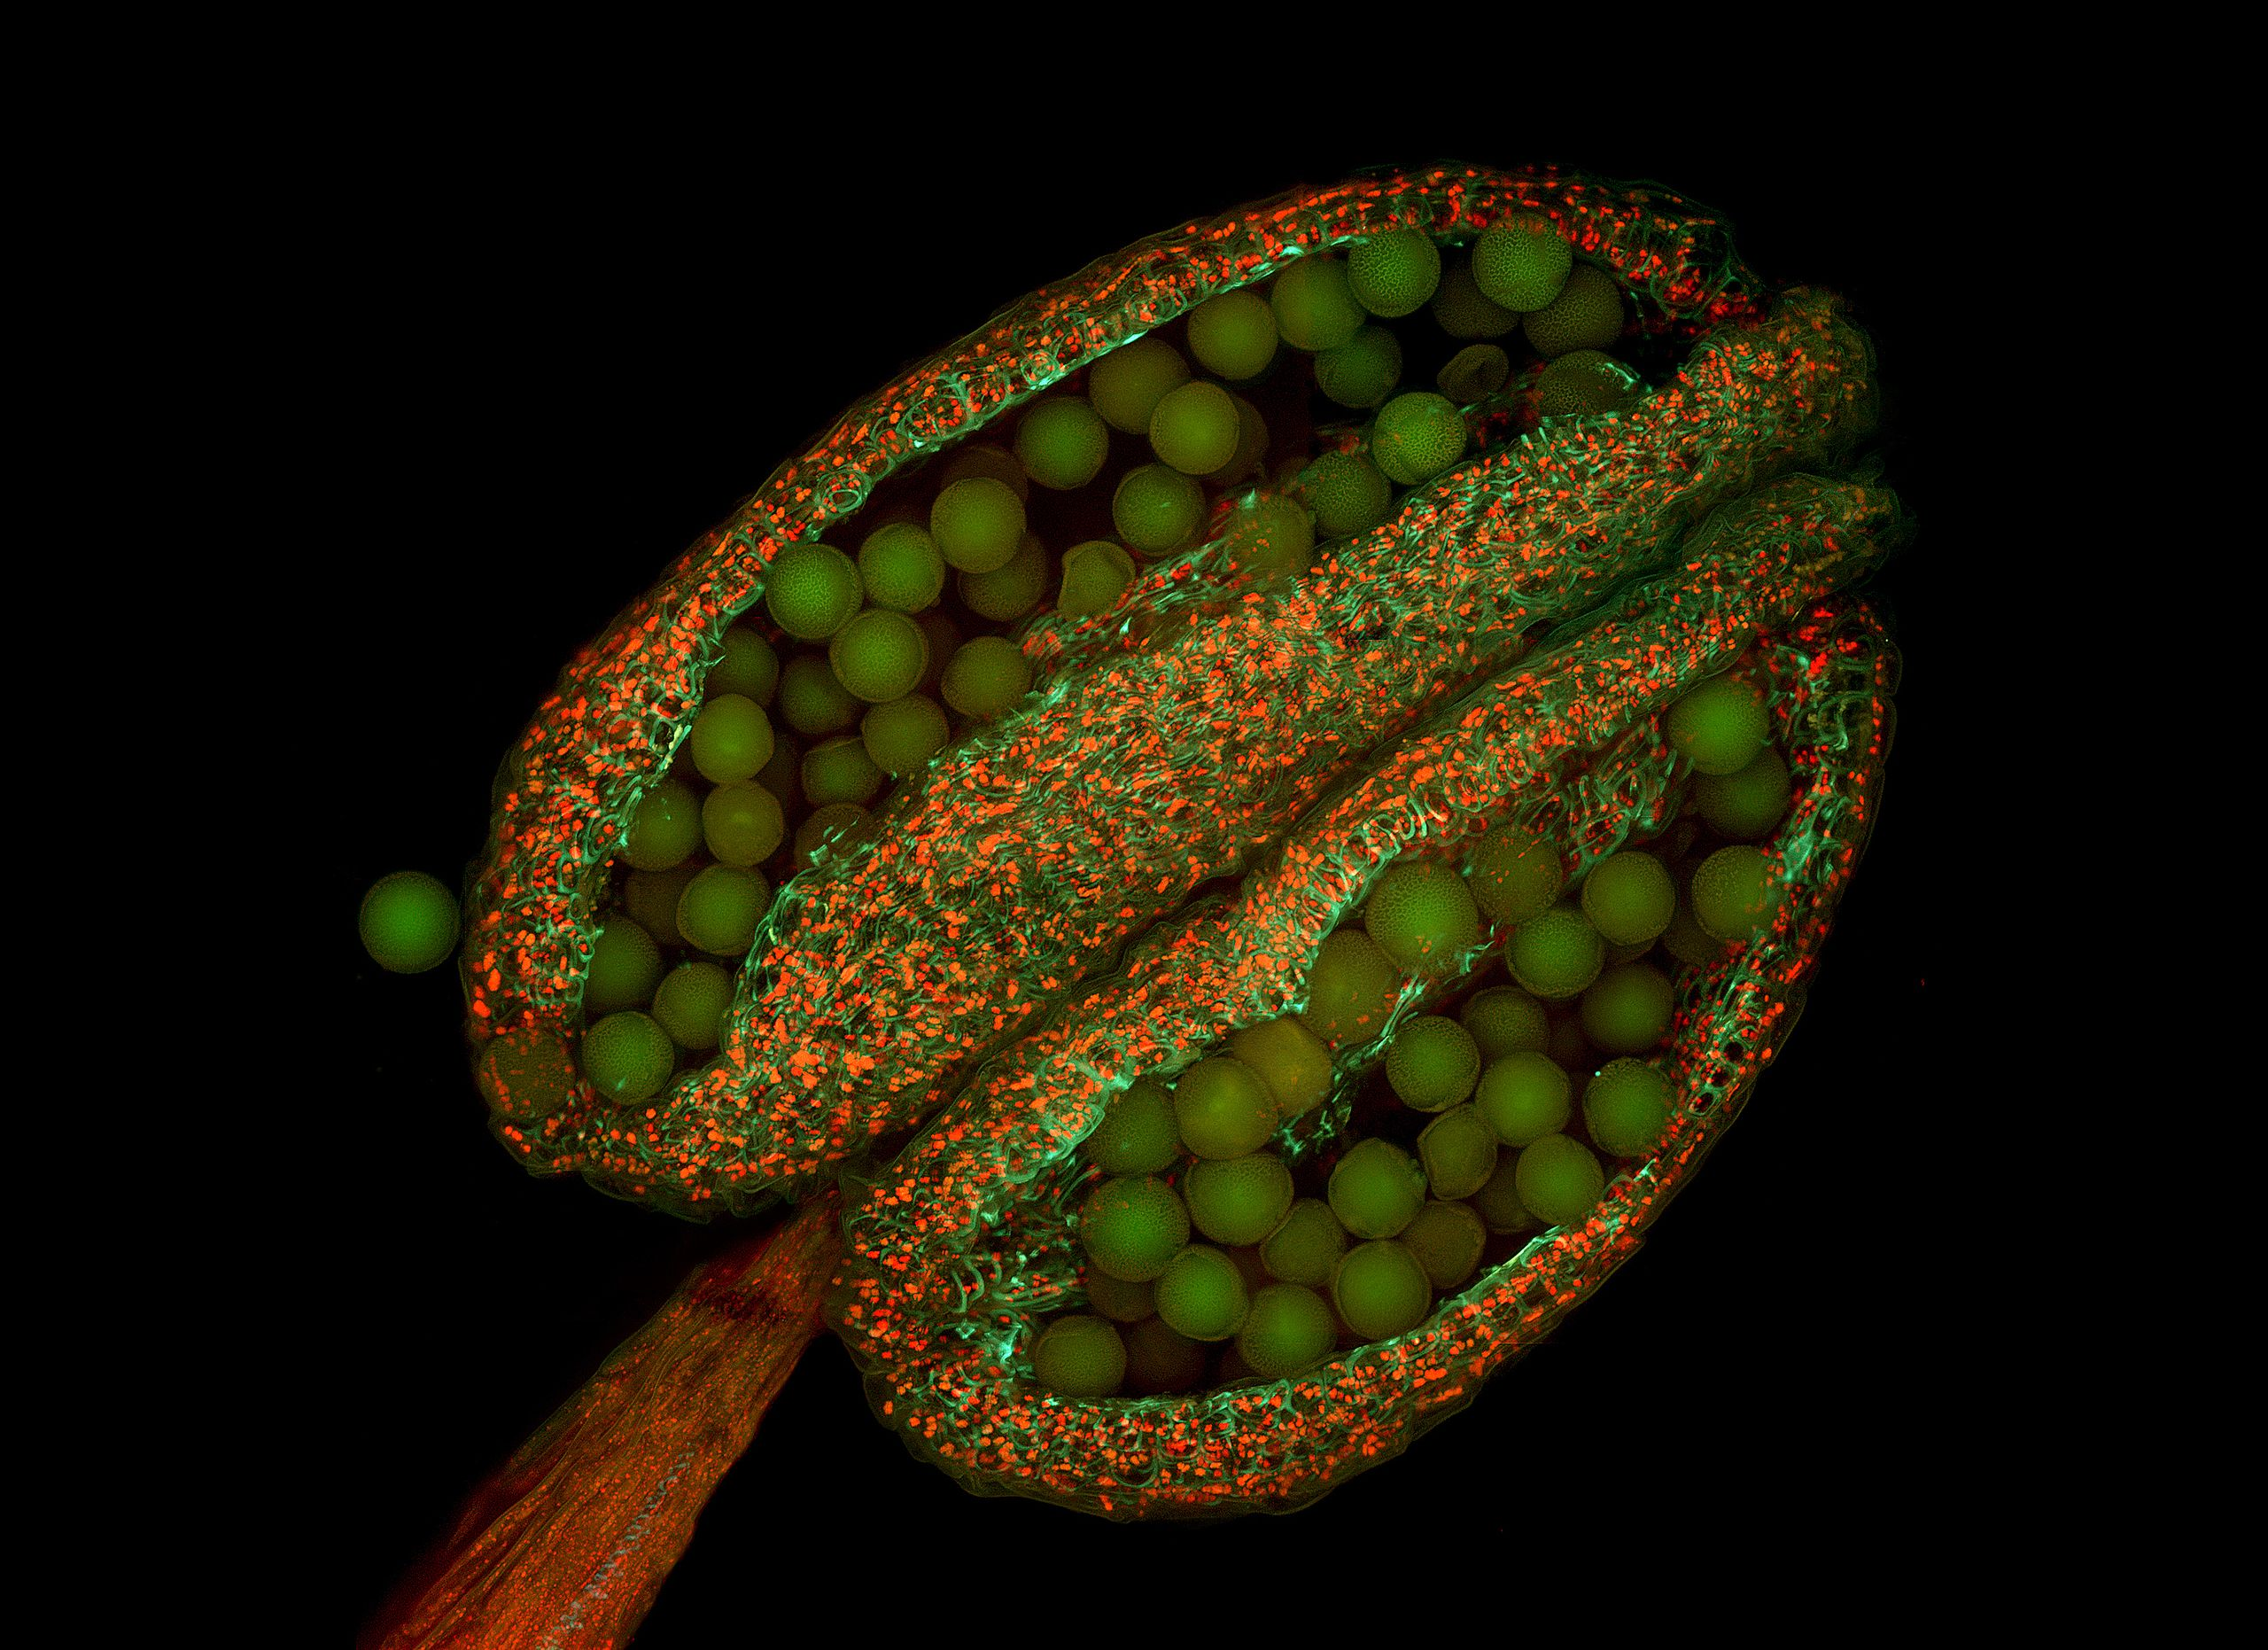
\includegraphics[width=\linewidth]{Tolmukapea.jpg}
% 	\caption{Anther of thale cress (Arabidopsis thaliana), fluorescence micrograph. Source: Heiti Paves, \href{https://commons.wikimedia.org/wiki/File:Tolmukapea.jpg}{https://commons.wiki-\\media.org/wiki/File:Tolmukapea.jpg}.}
% 	\label{fig:tcanther}
% \end{figure}

% Referencing a figure using its label: Figure \ref{fig:tcanther}.

% Aenean porttitor eros non pharetra congue. Proin in odio in dolor luctus auctor ac et mi. Etiam euismod mi sed lectus fringilla pretium. Phasellus tristique maximus lectus et sodales. Mauris feugiat ligula quis semper luctus. Nam sit amet felis sed leo fermentum aliquet. Mauris arcu dui, posuere id sem eget, cursus pulvinar mi. Donec nec lacus non lectus fermentum scelerisque et at nibh. Sed tristique, metus ac vestibulum porta, tortor lectus placerat lorem, et convallis tellus dolor eget ante. Pellentesque dui ligula, hendrerit a purus et, volutpat tempor lectus. Mauris nec purus nec mauris rhoncus pellentesque. Quisque quis diam sed est lacinia congue. Donec magna est, hendrerit sed metus vel, accumsan rutrum nibh.

% \begin{figure*} % Two column figure (notice the starred environment)
% 	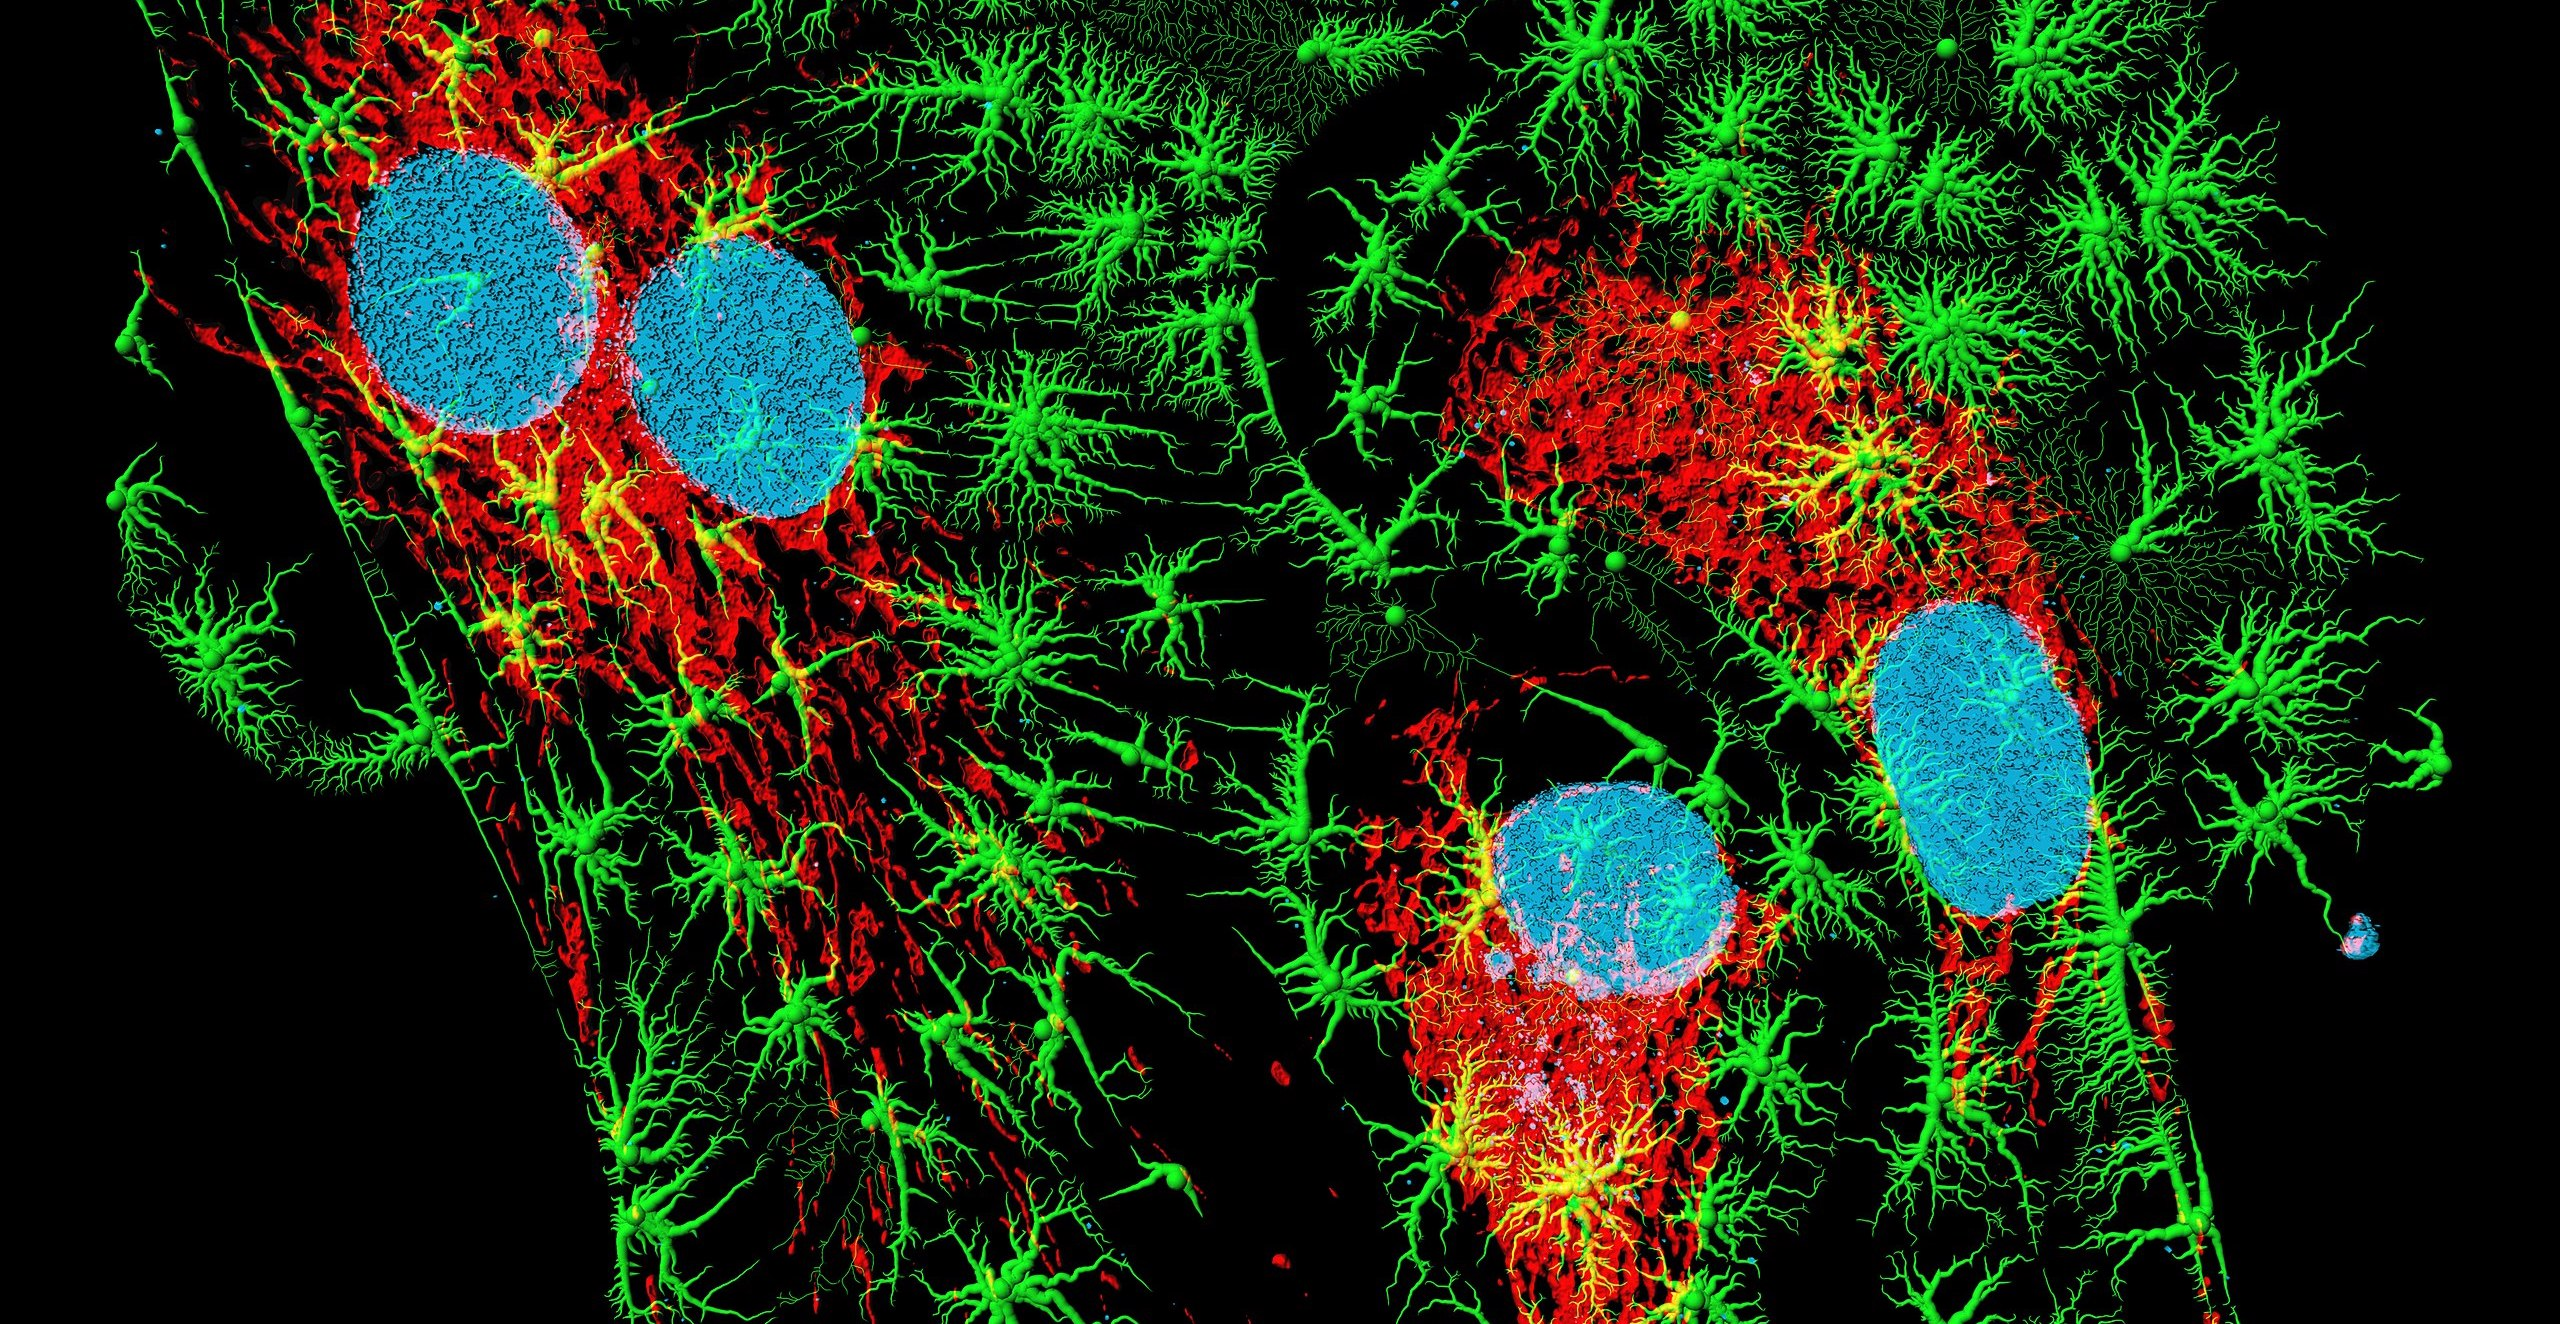
\includegraphics[width=\linewidth]{Fibroblastid.jpg}
% 	\caption{Bovine pulmonary artery endothelial cells in culture. Blue: nuclei; red: mitochondria; green: microfilaments. Computer generated image from a 3D model based on a confocal laser scanning microscopy using fluorescent marker dyes. Source: Heiti Paves, \href{https://commons.wikimedia.org/wiki/File:Fibroblastid.jpg}{https://commons.wikimedia.org/wiki/File:Fibroblastid.jpg}.}
% 	\label{fig:bpartery}
% \end{figure*}

% Orci varius natoque penatibus et magnis dis parturient montes, nascetur ridiculus mus. Etiam cursus lectus purus, tempus iaculis quam dictum tristique. Nam interdum sapien nec tempor mattis. Quisque id sapien nisi. Mauris vehicula ornare eros vel efficitur. Nulla consectetur, turpis quis fringilla tincidunt, mi neque iaculis lectus, vel commodo elit odio non ex. Duis facilisis, purus ac viverra iaculis, turpis lectus ultrices ante, ac vestibulum ligula magna in libero. Etiam tristique maximus lacinia. Vestibulum hendrerit, lacus malesuada laoreet blandit, sapien velit sollicitudin nunc, eu porttitor urna ligula at lorem. Aliquam faucibus eros in fermentum venenatis. Fusce consectetur congue pellentesque. Suspendisse at nisi sit amet est porttitor cursus. Cras placerat faucibus nunc, a laoreet justo dignissim sit amet.

% \subsection{International Support}

% \noindent àáâäãåèéêëìíîïòóôöõøùúûüÿýñçčšž

% \noindent ÀÁÂÄÃÅÈÉÊËÌÍÎÏÒÓÔÖÕØÙÚÛÜŸÝÑ

% \noindent ßÇŒÆČŠŽ

% \subsection{Links}

% This is a clickable URL link: \href{https://www.latextemplates.com}{LaTeX Templates}. This is a clickable email link: \href{mailto:vel@latextemplates.com}{vel@latextemplates.com}. This is a clickable monospaced URL link: \url{https://www.LaTeXTemplates.com}.

%------------------------------------------------
